\documentclass[../thesis.tex]{subfiles}

\begin{document}

\chapter{Details of minor backgrounds}
\label{chap:bkgDetails}

For the interested reader, we provide here a review of the studies undertaken within the Daya Bay Collaboration to determine the rate and spectra of three minor correlated backgrounds: fast neutrons, AmC backgrounds, and $\CanO$ reactions. As discussed in Sections~\ref{sec:bkgFastn}--\ref{sec:bkgCanO}, we use the results of these studies in order to these backgrounds from our sample of IBD candidates. This appendix also contains a discussion of uncorrelated instrumental (``flasher'') backgrounds, which are removed during the IBD pre-selection (\autoref{sec:selPreSel}). We begin with the flashers.

\section{PMT light emission (``flashers'')}
\label{sec:bkgFlashers}

During detector commissioning, most PMTs were found to occasionally emit varying amount of light due to arcing in their bases. The rate and intensity of this ``flashing'' would change over time for each PMT. At any given moment, some 5\% of the PMTs in each AD will have the tendency to flash brightly enough to trigger the detector \cite{SideBySide}, in some cases producing as much as 100~MeV of reconstructed energy. Within the delayed energy region of 6-12~MeV, the flasher rate has averaged at around 0.7~Hz for each AD. These ``delayed-like'' flashers, if included in the analysis, would significantly increase the rate of backgrounds caused by the accidental coincidence of two uncorrelated signals. As discussed in \autoref{sec:accbkg} and \autoref{chap:accDMC}, the rate of such ``accidentals'' is proportional to the rate of delayed-like signals, and this rate (excluding flashers) ranges from around 0.05~Hz at EH3 to 1~Hz at EH1. While the flashers would merely (roughly) double the 1\% accidental background in the near halls, in the far hall it would increase this background by an order of magnitude to the 10\% level, counter to Daya Bay's goal of perecent-level background contamination.

Fortunately, flashers are easily distinguished from ``physical'' singles due to their unique pattern of light emission, enabling them to be removed from the analysis with high efficiency while minimally affecting true IBDs. This light pattern is characterized by two ``hot spots'' on opposite sides of the AD. When a PMT base emits light, much of the light is absorbed by the black radial shield and the conical magnetic shield. The remainder escapes within a conical profile; some of the photons will strike the flasher's photocathode (resulting in the flashing PMT having the highest charge), and others will primarily illuminate the PMTs across the AD from the flasher, especially the one that lies directly opposite to it. In addition, the time distribution of the PMT hits is broadened for flashers due to the geometry of light propagation across the AD. By taking advantage of these telltale distributions of charges and times, it is possible to achieve excellent discrimination of flashers from physical events.

The flasher identification criteria were developed in a somewhat ad-hoc fashion, by defining quantities that could conceivably serve as discriminators, and then further defining combinations of these quantities, and finally plotting the distributions of these (combined) quantities until a clean separation between flashers and non-flashers was apparent. It is far more important to minimize (IBD) signal inefficiency instead of maximizing flasher rejection, because a small amount of unrejected flashers will simply slightly increase the rate of accidental backgrounds (which can be easily quantified), whereas a signal inefficiency could vary among the ADs and thereby bias the oscillation fit.

Early in the experiment, this prolonged and iterative process eventually gave rise to the \emph{ellipse cut} (based on the charge distribution) and the \emph{PSD cut} (based on the time distribution), which demonstrated excellent performance, and these cuts continue to be used in this analysis. The ellipse cut is based on two quantities, termed $\fmax$ and $\fquad$. The first, $\fmax$, is simply the ratio of $Q_{\mathrm{max}}$ (the maximum individual PMT charge across all PMTs) over the total charge $Q_{\mathrm{tot}}$:
\begin{equation}
  \fmax = \frac{Q_{\mathrm{max}}}{Q_{\mathrm{tot}}}.
\end{equation}
For flasher events, $Q_{\mathrm{max}}$ belongs to the flashing PMT itself, and $\fmax$ is typically higher for flashers than for physics events. However, physical events near the PMTs can exhibit high $\fmax$, so this variable alone is insufficient to cleanly discriminate flashers. As such, we also consider $\fquad$, which is based on dividing the AD into four quadrants (\autoref{fig:flasher_example}): ``Quadrant 1'' (q1) is the one that is centered on the highest-charge PMT, q3 is the one across from q1, and q2 and q4 are the two ``to the side.'' Then, $\fquad$ captures the conical nature of the light emission:
\begin{equation}
  \fquad = \frac{Q_{\mathrm{q3}}}{Q_{\mathrm{q2}} + Q_{\mathrm{q4}}}.
\end{equation}
Like $\fmax$, $\fquad$ alone is not a good discriminator, due to overlap between flashers and physics events. However, their combination
\begin{equation}
  \fID = \log_{10} \left[ \fquad^2 + \left( \frac{\fmax}{0.45} \right)^2 \right]
\end{equation}
turns out to be an excellent discriminator. Indeed, as shown by \Autoref{fig:fID_dist,fig:bkgFlasherEllipse2D}, requiring
\begin{equation}
  \label{eq:ellipseCut}
  \fID < 0
\end{equation}
reduces the flasher rate to a negligible level, and many analyses have relied on $\fID$ alone to identify flashing 8" PMTs.

\begin{figure}[h]
  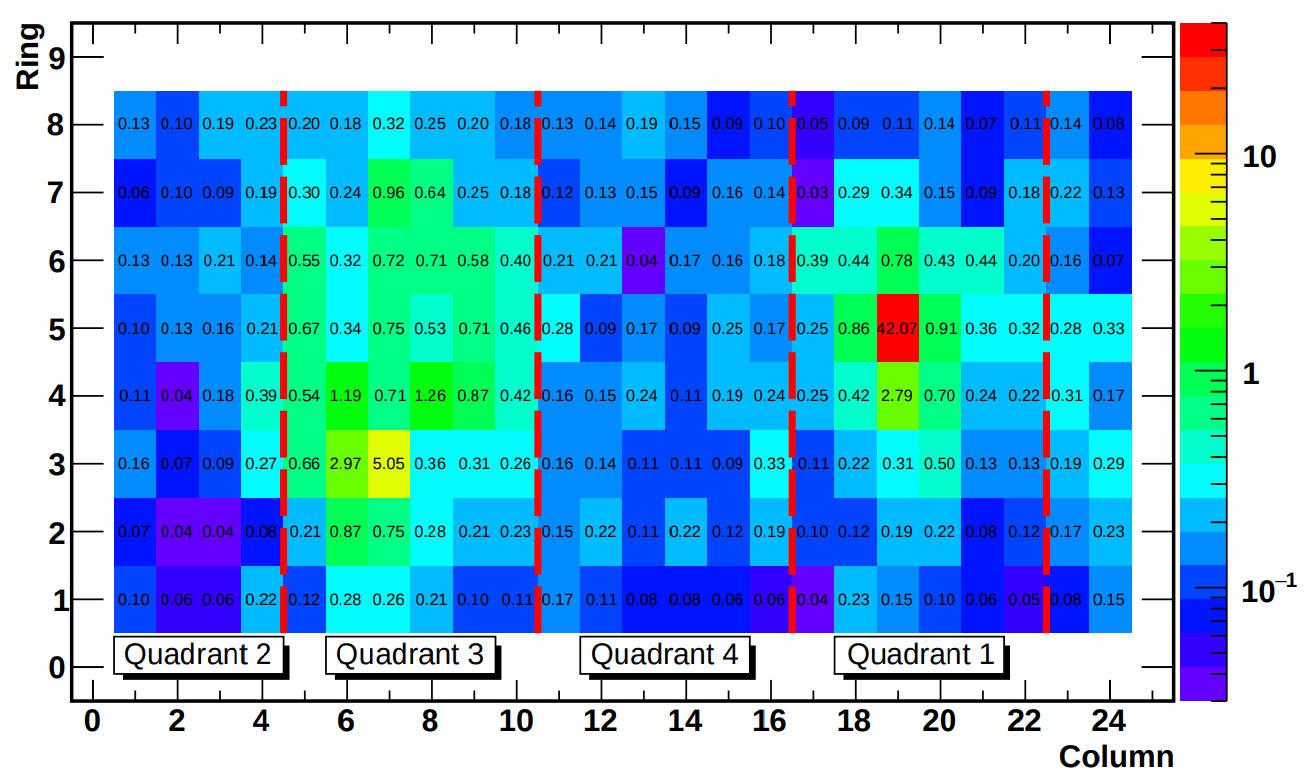
\includegraphics[width=\textwidth]{Backgrounds/Flasher/example_event.png}
  \caption{PMT charge distribution of a flasher candidate, illustrating the division of the AD into four azimuthal quadrants, with Quadrant 1 being centered around the PMT with the highest charge. From \cite{An_2017}.}
  \label{fig:flasher_example}
\end{figure}

\begin{figure}[h]
  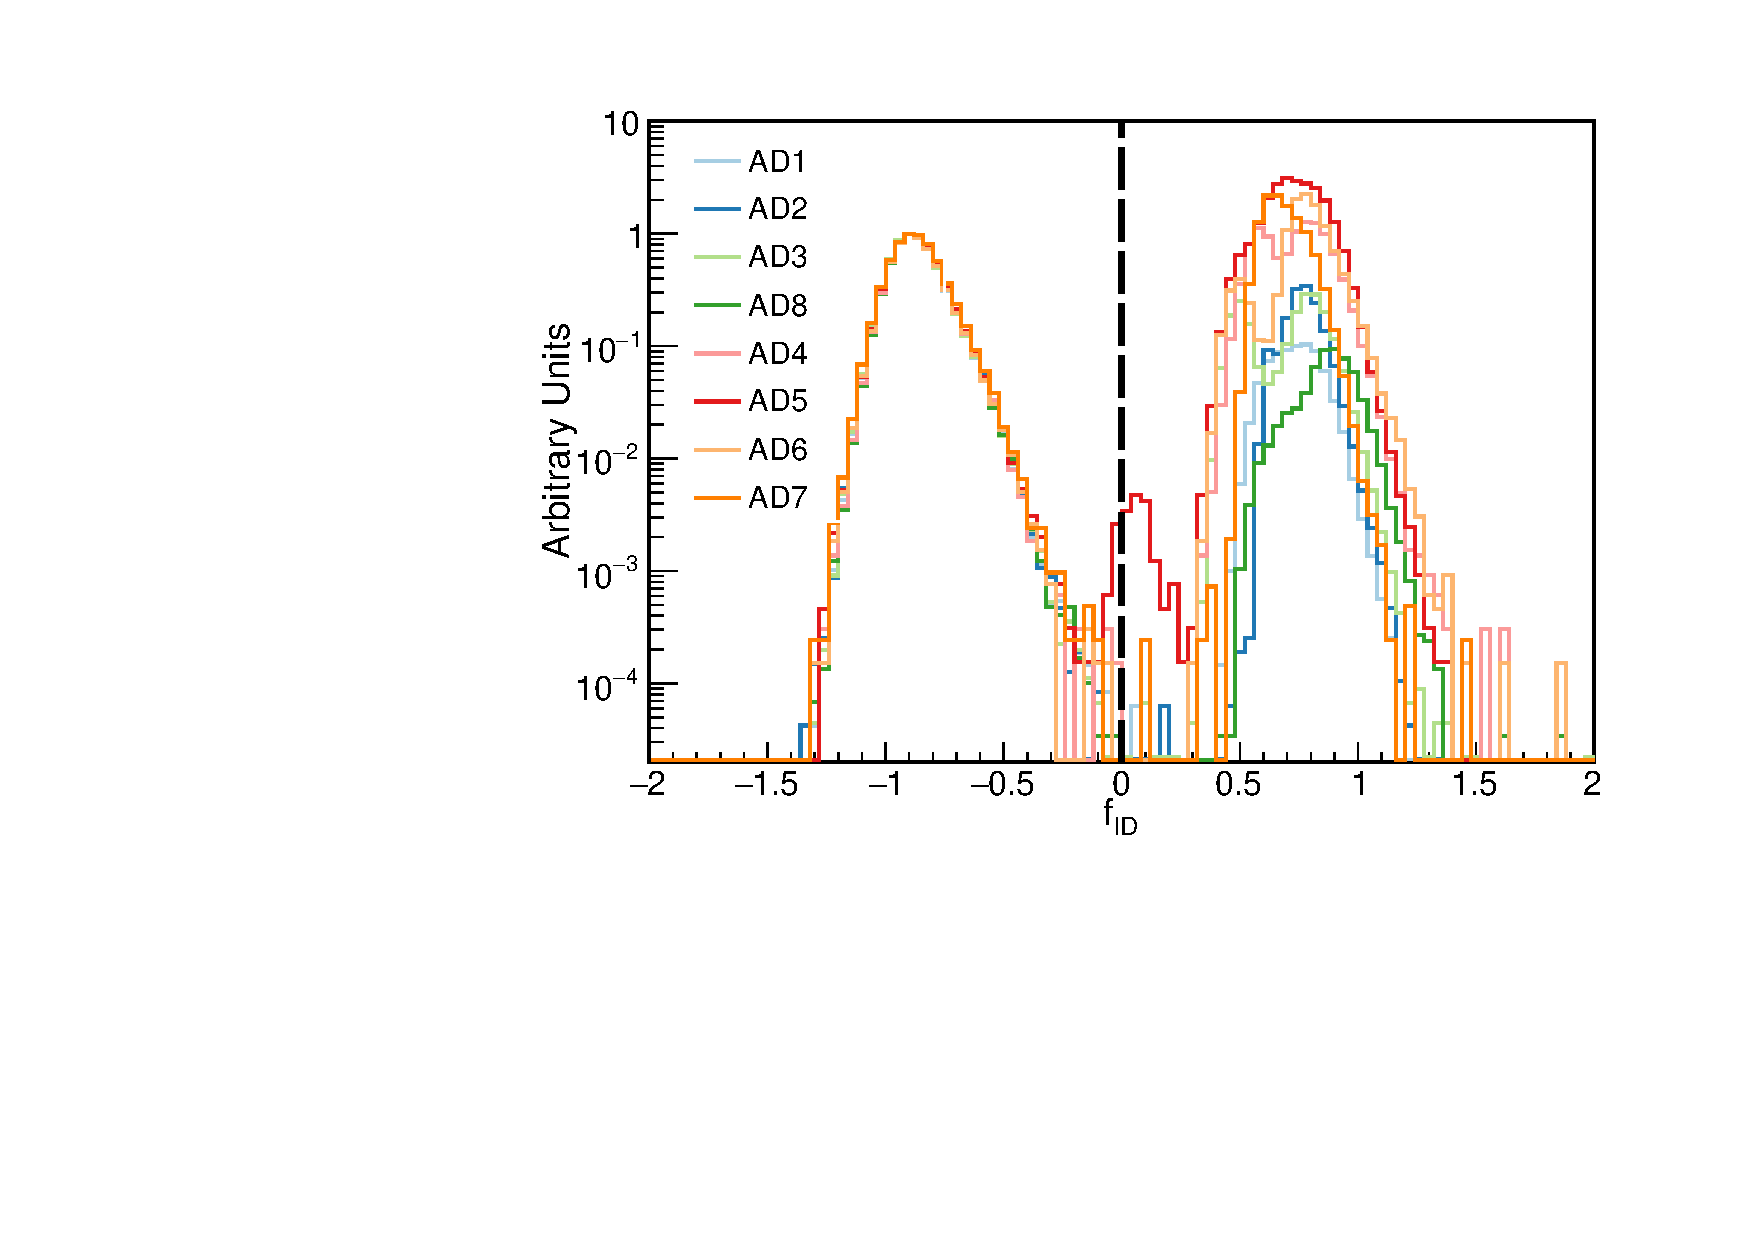
\includegraphics[scale=0.5]{Backgrounds/evt_flasherFID_Delayed.pdf}
  \caption{Distribution of the flasher discriminator $\fID$ for the delayed triggers of IBD candidates. The tagged flashers ($\fID > 0$) are cleanly separated from physics signals, with the exception of a single flasher in AD5 which leaked into the signal region (leading to a slight increase in the singles rate). In all ADs, there is essentially no signal lost. From \cite{An_2017}.}
  \label{fig:fID_dist}
\end{figure}

\begin{figure}[ht!]
  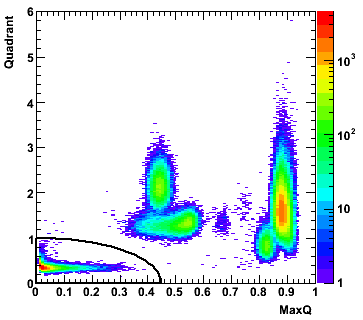
\includegraphics[width=0.5\textwidth]{Backgrounds/Flasher/ellipse_2d.png}
  \caption{Two-dimensional distribution of $\fmax$ (``MaxQ'') and $\fquad$ (``Quadrant'') for physical triggers in EH1-AD2. The black ``ellipse'' corresponds to $\fID = 0$; events outside the ellipse are identified as flashers. High flasher rejection and negligible signal inefficiency are apparent. From \cite{flasherControl}.}
  \label{fig:bkgFlasherEllipse2D}
\end{figure}

Even further flasher reduction can be achieved by incorporating timing information. To capture the broadening of the time distribution shown by flashers, we use the variable(s) $f_{\mathrm{t}1}$ ($f_{\mathrm{t}2}$), defined as the ratio of the number of hits in the first 200 (150)~ns of the signal, over the number of hits in the first 400~ns. The discriminator $\fPSD$ is then defined as
\begin{equation}
  \fPSD = \log_{10} [4 \cdot (1 - f_{\mathrm{t}1})^2 + 1.8 \cdot (1 - f_{\mathrm{t}2})^2].
\end{equation}
By requiring both $\fID < 0$ and $\fPSD < 0$, we eliminate virtually all 8" PMT flashers from the analysis.

However, in addition to the 192 8" PMTs, there are six 2" PMTs located at the top and bottom of each AD along the calibration axes, and these can also flash. Such events were easily identified as those in which any 2" PMT saw an extreme amount of charge, with a cut of 100 PE providing essentially perfect separation between 2" PMT flashers and other events.

\section{Cosmogenic fast neutrons}
\label{sec:bkgFastn}

\subsection{Event selection}
\label{sec:fastn_sel}

Two event samples are used in the fast-neutron analysis. The first, which we shall refer to as the ``untagged'' sample, is obtained using the standard IBD selection, as described in \autoref{chap:selection}, with the modification that the upper limit on the prompt energy is extended to 300~MeV instead of the usual 12~MeV. In this sample, the prompt spectrum below 12~MeV is essentially the same as the one used in the oscillation fit (i.e., dominated by true IBDs), whereas the high-energy region almost exclusively contains the (recoil protons from) fast-neutron events.

The other, ``tagged,'' sample contains IBD-like events that occur right after a muon that triggers \emph{only} the outer water pool. When a muon passes through the AD or the IWS, the resulting spallation products generate a significant amount of prompt activity in the AD. On the other hand, when a muon triggers only the OWS, without involvement of the IWS or AD, most of the debris is unable to penetrate into the GdLS. Fast neutrons, however, are an exception. The OWS tagging therefore provides a highly pure sample of fast neutrons for analysis.

The tagged sample is obtained by extending the upper cut to 300~MeV (as in the untagged sample) while disabling the standard muon veto. An additional requirement (see \autoref{fig:fastn_selection_diagram}) is that the prompt signal be timestamped within (-300, 600)~ns of an OWS trigger (defined by NHit $>$ 15, in this case). Furthermore, the delayed signal must occur at least 15 $\mu$s after the muon in order to eliminate Michel electrons, and there must be no AD or IWS muons within 600~\us\ of the OWS muon. This selection results in fairly low statistics (amounting to a few hundred events in the near halls), but the size of the sample is still sufficient to provide strong constraints on the fast-neutron background. This sample is statistically independent from the untagged sample, as all of its events would have been excluded by the (OWS) muon veto in the untagged selection.

\begin{figure}[h]
  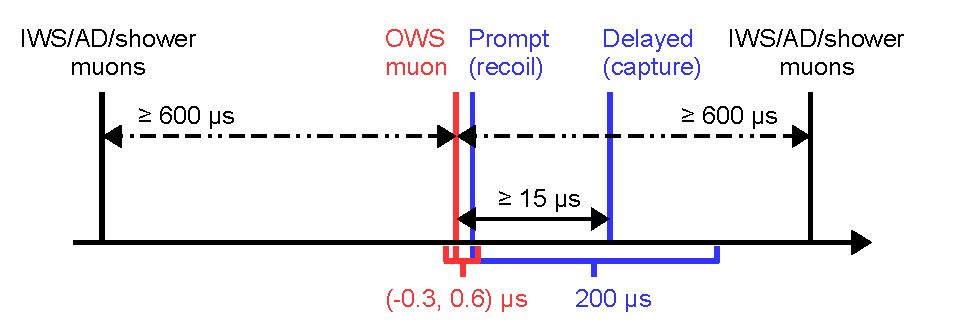
\includegraphics[width=0.9\textwidth]{Backgrounds/FastN/fastn_diagram_mine.pdf}
  \caption{Diagram illustrating the event selection scheme for the tagged fast-neutron sample.}
  \label{fig:fastn_selection_diagram}
\end{figure}

The prompt spectra from the two samples (scaled to have equal normalization above 12~MeV) are overlaid in \autoref{fig:fastn_prompt_energy_both_bz}, showing excellent agreement in the region between 12 and 150~MeV. Both samples are employed by the scaling method, as described next. Meanwhile, the extrapolation method only makes direct use of the tagged sample; however, the untagged sample still serves a role in validating the form of the fitting function used.

\begin{figure}[h]
  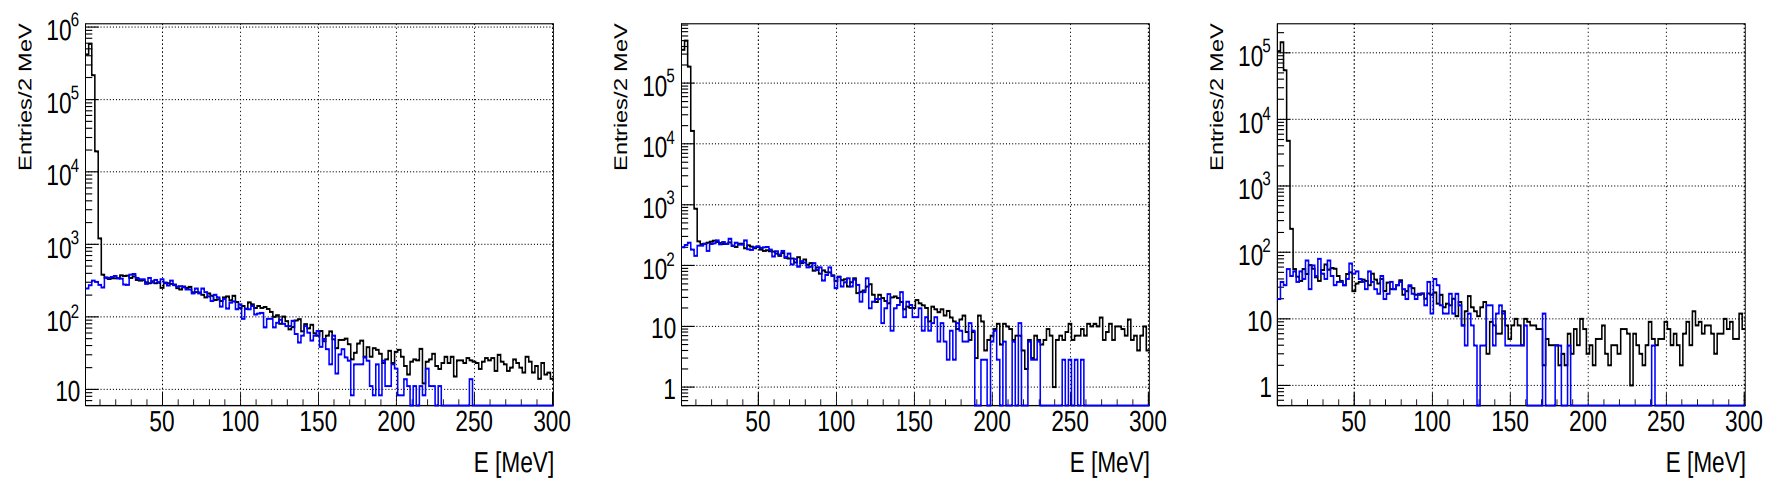
\includegraphics[width=\textwidth]{Backgrounds/FastN/prompt_energy_both_bz.png}
  \caption{Prompt spectra of the tagged (blue) and untagged (black) samples. The tagged spectrum has been rescaled to match the normalization of the untagged spectrum above 12~MeV. From \cite{fastn}.}
  \label{fig:fastn_prompt_energy_both_bz}
\end{figure}

\subsection{Scaling method}
\label{sec:fastn_scaling}

In the scaling method, we assume that the shape of the tagged spectrum is an accurate representation of the shape of the fast-neutron background. In other words, we assume that, for any given fast neutron, there is no energy dependence on the probability of its association with an OWS-only muon. Previous studies within the collaboration have supported the validity of this assumption.

\def\emax{\ensuremath{E_\mathrm{max}}} \def\ntag{\ensuremath{N_\mathrm{tag}}}
\def\nuntag{\ensuremath{N_\mathrm{untag}}}

We define the \emph{scaling factor} $F$ as
\begin{equation}
  F(\emax) = \frac{\nuntag[12, \emax]}{\ntag[12, \emax]},
\end{equation}
i.e., the ratio of the integral of the two samples between 12~MeV and \emax. The dependence on \emax\ reflects the arbitrary choice of the upper energy limit, which contributes to the uncertainty on the result (primarily due to statistical fluctuations in the small sample of tagged neutrons). This uncertainty is quantified by comparing the results for \emax\ of 80, 100, 120, and 150~MeV (\autoref{fig:fastn_scaling_factor}) \cite{fastn} , resulting in an estimated systematic uncertainty given by the half-range divided by the mean, as listed in \autoref{tab:bkgFastnUnc}. In addition, for a \emph{fixed} \emax, there is a purely statistical uncertainty\footnote{As noted previously, the tagged and untagged samples are statistically independent.},
\begin{equation}
  \sigma_F(\emax) = F \cdot \sqrt{\nuntag^{-1}[12, \emax] + \ntag^{-1}[12,
      \emax]},
\end{equation}
which also contributes to the final uncertainty.

\begin{figure}[h]
  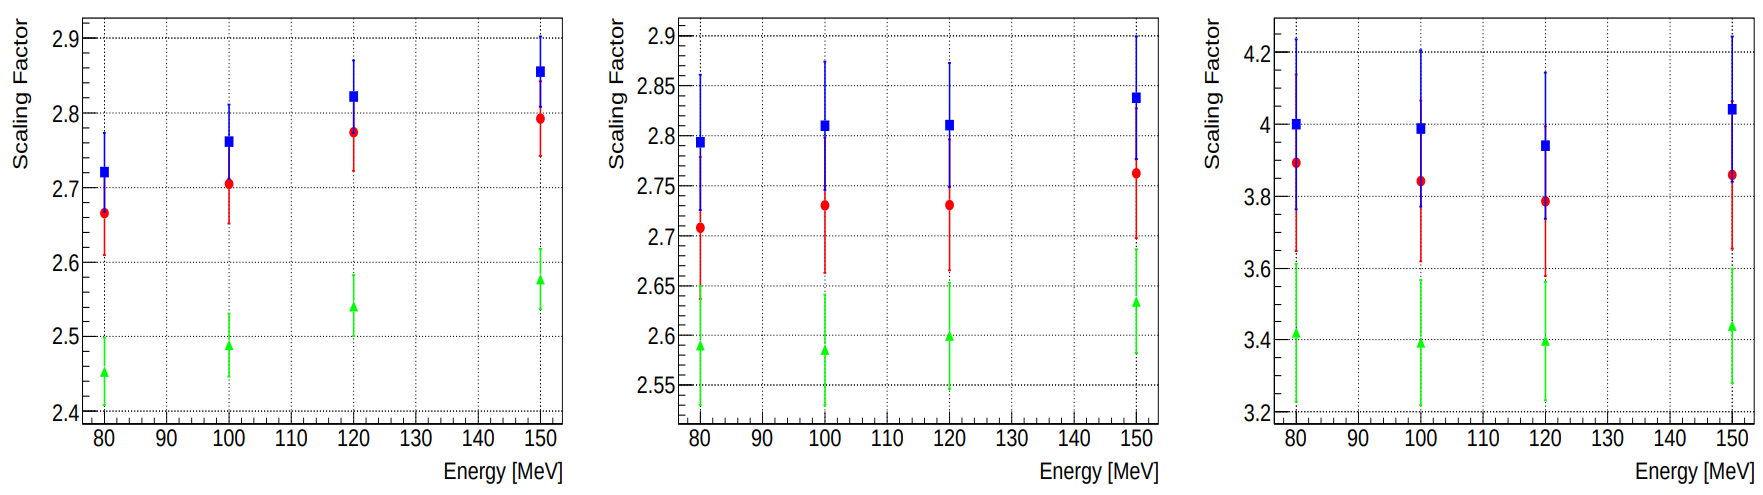
\includegraphics[width=\textwidth]{Backgrounds/FastN/scaling_factor.png}
  \caption{Comparison of the scaling factor $F(E_{\mathrm{max}})$ obtained for different values of $E_{\mathrm{max}}$. The three colors correspond to different IBD selection criteria, with the blue squares representing the criteria used in this analysis. From \cite{fastn}.}
  \label{fig:fastn_scaling_factor}
\end{figure}

\def\nfn{\ensuremath{N_\mathrm{FN}}} \def\rfn{\ensuremath{R_\mathrm{FN}}}

For the standard IBD selection, the number of fast neutrons within the fiducial energy range of [0.7, 12]~MeV is determined simply as
\begin{equation}
  \nfn = F \cdot \ntag[0.7, 12].
\end{equation}
Its statistical uncertainty, in turn, is
\begin{equation}
  \label{eq:fastn_scal_unc}
  \sigma_\mathrm{FN} = \sqrt{\ntag^2[0.7, 12]
    \cdot \sigma_F^2 + F^2 \cdot \ntag[0.7, 12]}.
\end{equation}
Finally, the normalized daily fast-neutron rate is
\begin{equation}
  \label{eq:fastn_rate}
  \rfn = \frac{\nfn}{T_\mathrm{DAQ} \cdot \epsilon_\mu \cdot \epsilon_m},
\end{equation}
where $T_\mathrm{DAQ}$, $\epsilon_\mu$, and $\epsilon_m$ are the DAQ livetime, muon veto efficiency, and multiplicity cut efficiency for the untagged sample. The resulting $\rfn$, for the four different values of $E_{\mathrm{max}}$, are plotted in \autoref{fig:fastn_rate_vs_scaling}.

% This value is then combined with the extrapolation result, described next, and a total uncertainty is assigned to the combination.

\begin{figure}[h]
  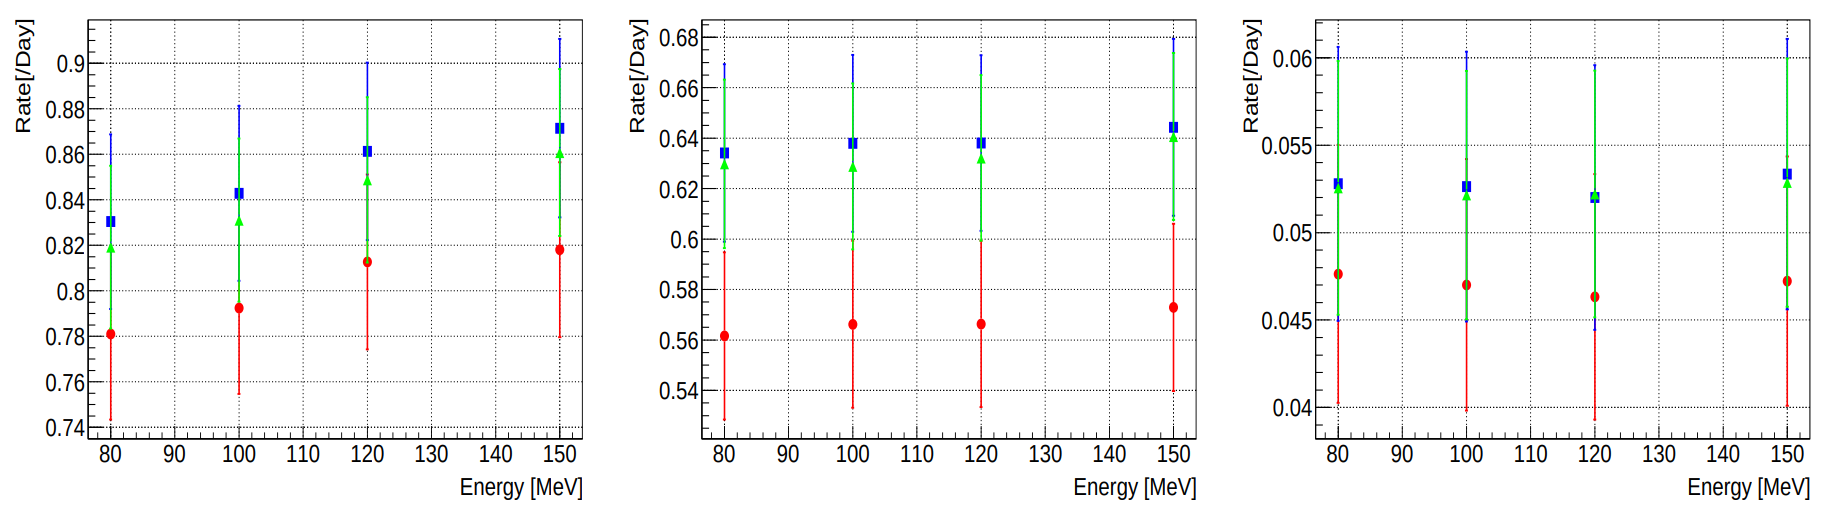
\includegraphics[width=\textwidth]{Backgrounds/FastN/rate_vs_scaling.png}
  \caption{Daily fast-neutron rate from the scaling method, as a function of $E_{\mathrm{max}}$. The blue squares correspond to the IBD selection criteria used in this analysis. From \cite{fastn}.}
  \label{fig:fastn_rate_vs_scaling}
\end{figure}

\subsection{Extrapolation method}
\label{sec:fastn_extrap}

Previous simulation studies have found that the fast neutron spectrum can be accurately described by the PDF
\begin{equation}
  \label{eq:bkgFastnShape}
  f(E; E_0, a) = A \cdot \left( \frac{E}{E_0} \right)^{-a-E/E_0},  
\end{equation}
where $E_0$ and $a$ are shape parameters, and $A(E_0, a)$ normalizes the PDF. When a measured fast-neutron spectrum is then fit to the form
\begin{equation}
  \label{eq:bkgFastnScaledPDF}
  S(E; N, E_0, a) = N \cdot f(E; E_0, a),
\end{equation}
the best-fit value of $N$ represents the number of events ``under the curve'' from 0 to $\infty$~MeV.

In turn, if we have a (hypothetical) pure fast-neutron spectrum containing $\nfn$ events in the fiducial region of [0.7, 12]~MeV, then the full spectrum ([0, $\infty$]~MeV) should contain an event count equal to
\begin{equation}
  N = \frac{\nfn}{\int_{0.7}^{12} f(E; E_0, a)\,dE }.
\end{equation}
Here, the denominator represents the fiducial region's fraction of the total spectrum. Substituting this form of $N$ into \autoref{eq:bkgFastnScaledPDF}, and allowing the floated parameter to be $\nfn$ instead of $N$, we obtain the form
\begin{equation}
  \label{eq:fastn_extrap_form}
  S(E; \nfn, E_0, a) = \frac{\nfn}%
  {\int_{0.7}^{12} E'^{-a-E'/E_0} \, dE'} E^{-a-E/E_0}.
\end{equation}
When \autoref{eq:fastn_extrap_form} is then fit to the measured fast-neutron spectrum, the best-fit $\nfn$ indicates the number of events in the fiducial region. The key to the extrapolation method is that this fit is performed outside the fiducial region, where the fast-neutron sample is uncontaminated.

The validity and robustness of \autoref{eq:fastn_extrap_form} was verified by fitting it to the OWS-tagged samples from each hall (\autoref{fig:fastn_ows_fit_bz}) \cite{fastn}. Four fitting ranges were used, all starting at 0.7~MeV, and ending at 80, 100, 120, and 150~MeV. All fits produced satisfactory goodness-of-fit and consistent values of $E_0$ (\autoref{fig:fastn_par_E0_ows}). Disabling of the $a$ parameter was found to introduce negligible differences. As summarized in \autoref{tab:fastnShapePars}, we define the nominal value of $E_0$ to be the average from the eight fits in each hall (four fitting ranges, with and without $a$). This value is then inserted into \autoref{eq:bkgFastnShape} (with $a = 0$) to generate the spectral shape of the fast-neutron background. Normalizing this shape to the predicted fast-neutron rate then gives the prompt spectrum that we subtract from that of the IBD candidates.

\begin{figure}[ht]
  \begin{minipage}{0.333\textwidth}%
    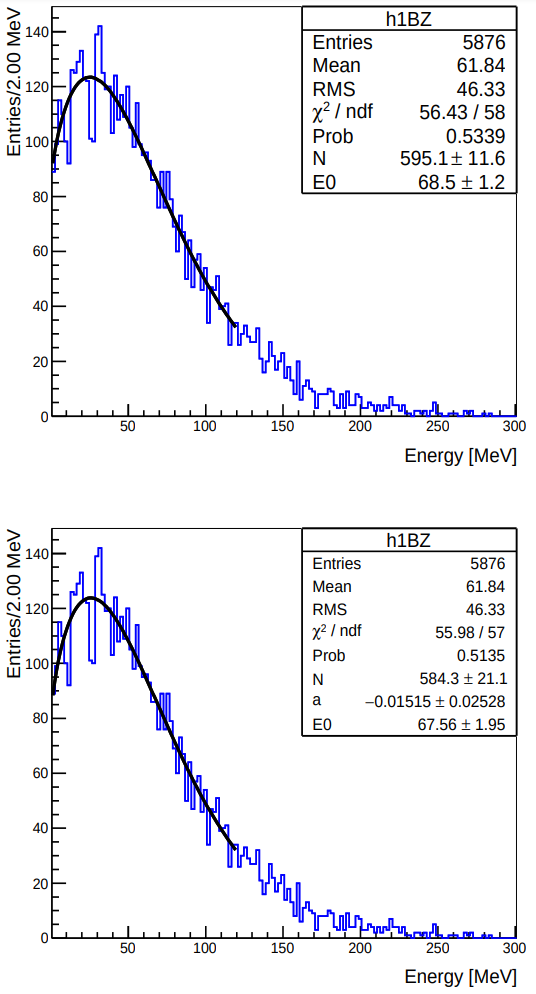
\includegraphics[width=\textwidth]{Backgrounds/FastN/ows_fit_eh1_bz.png}%
  \end{minipage}%
  \begin{minipage}{0.333\textwidth}%
    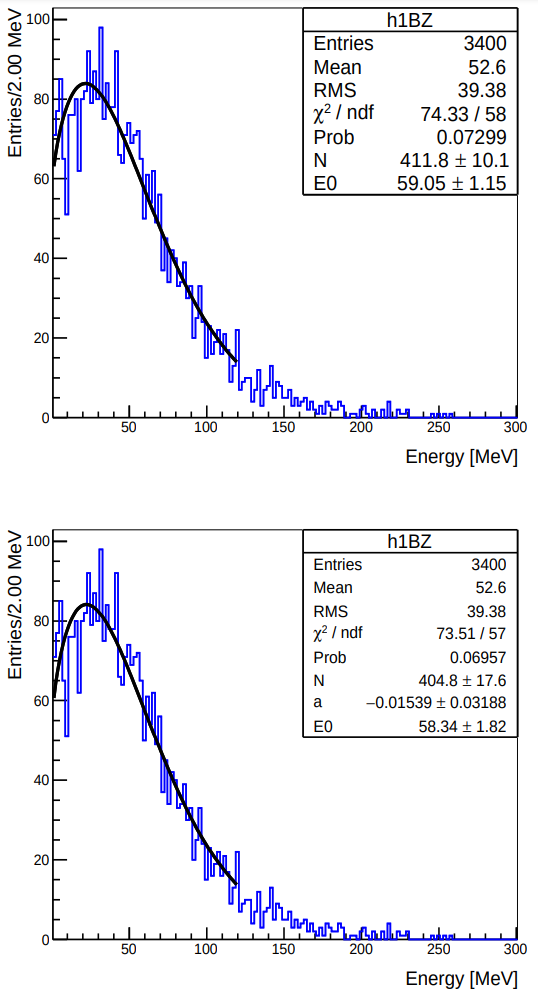
\includegraphics[width=\textwidth]{Backgrounds/FastN/ows_fit_eh2_bz.png}%
  \end{minipage}%
  \begin{minipage}{0.333\textwidth}%
    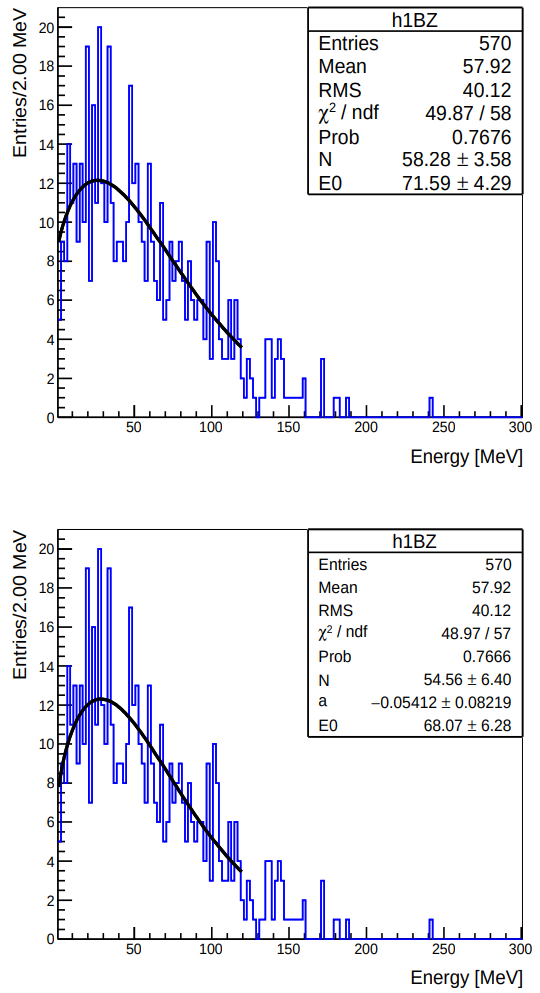
\includegraphics[width=\textwidth]{Backgrounds/FastN/ows_fit_eh3_bz.png}%
  \end{minipage}%
  \caption{Fits of the OWS-tagged fast-neutron spectra to \autoref{eq:fastn_extrap_form} for EH1 (left), EH2 (center), and EH3 (right). From \cite{fastn}.}
  \label{fig:fastn_ows_fit_bz}
\end{figure}

\begin{figure}[ht]
  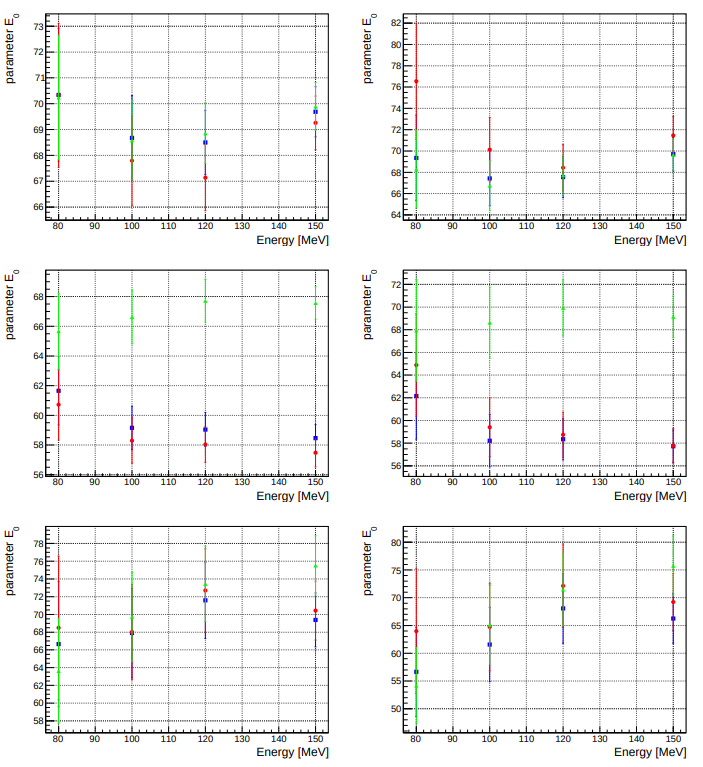
\includegraphics[scale=0.65]{Backgrounds/FastN/par_E0_ows.png}
  \caption{Values of the shape parameter $E_0$ obtained from fitting the OWS-tagged fast-neutron samples to \autoref{eq:fastn_extrap_form}. The parameter $a$ was fixed to zero for the plots on the left, while it was allowed to float for the plots on the right. The blue squares correspond to the IBD selection criteria used in this analysis; the average of the eight values for each hall, as reproduced in \autoref{tab:fastnShapePars}, is used when subtracting the fast-neutron background in our analysis. From \cite{fastn}.}
  \label{fig:fastn_par_E0_ows}
\end{figure}

\begin{table}[ht]
  \begin{tabular}{lc}
    \toprule
    Hall & $E_0$ (MeV) \\
    \midrule
    EH1 & 68.68 \\
    EH2 & 59.16 \\
    EH3 & 67.91 \\
    \bottomrule
  \end{tabular}
  \caption{Fast-neutron shape parameters $E_0$ (inserted into \autoref{eq:bkgFastnShape}) used for subtracting this background in each hall \cite{fastn}.}
    \label{tab:fastnShapePars}
\end{table}

Finally, the fit was performed on the untagged sample (\autoref{fig:fastn_ibd_fit_bz}), using the same four upper limits as before, but with the lower limit set to 12~MeV.  As with the scaling method, each value of $\nfn$ was converted to a livetime- and efficiency-normalized daily rate according to \autoref{eq:fastn_rate} (\autoref{fig:fastn_rate_vs_fit_range}). The spread between the resulting four values was incorporated into the total uncertainty, as described in the next section.

\begin{figure}[ht]
  \begin{minipage}{0.333\textwidth}%
    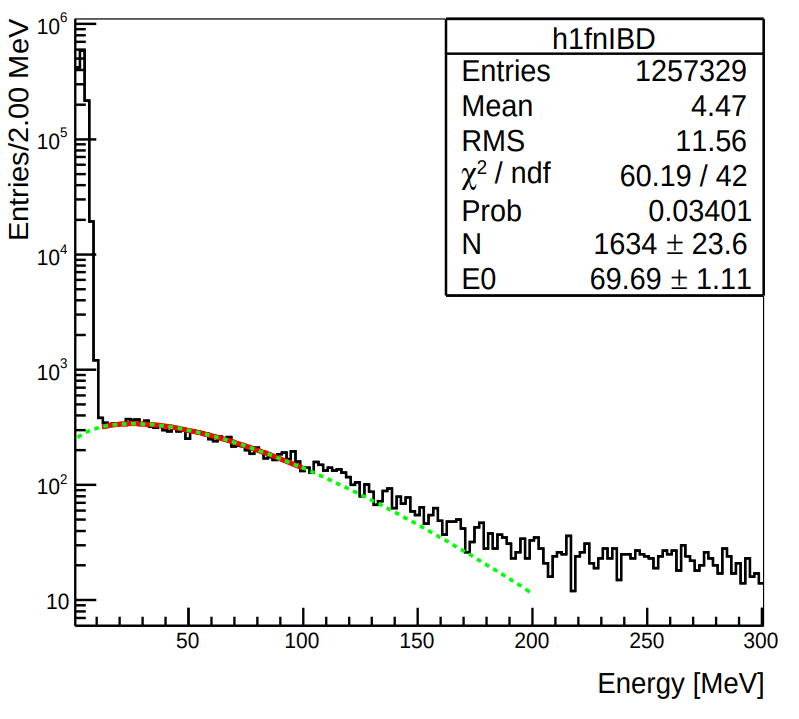
\includegraphics[width=\textwidth]{Backgrounds/FastN/ibd_fit_eh1_bz.png}%
  \end{minipage}%
  \begin{minipage}{0.333\textwidth}%
    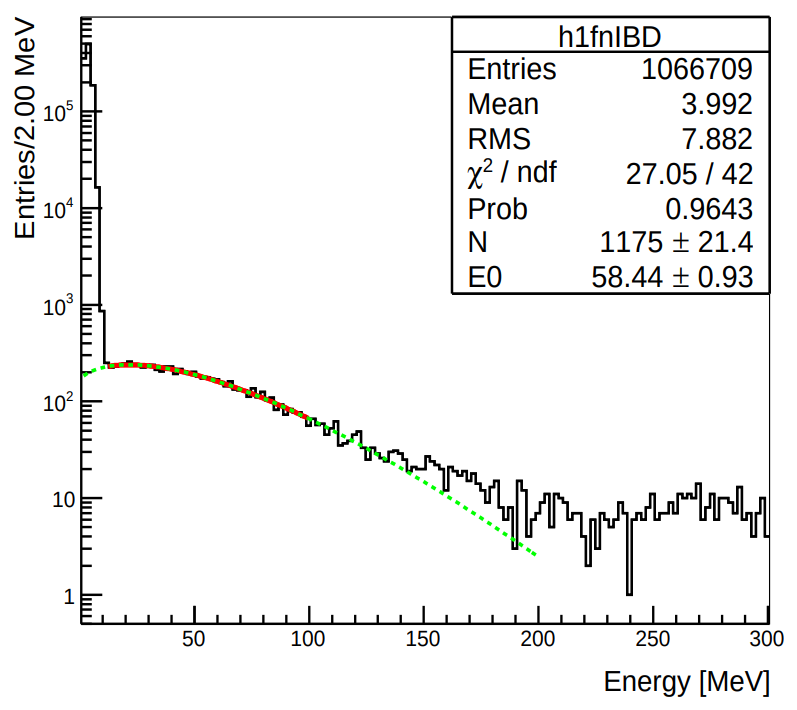
\includegraphics[width=\textwidth]{Backgrounds/FastN/ibd_fit_eh2_bz.png}%
  \end{minipage}%
  \begin{minipage}{0.333\textwidth}%
    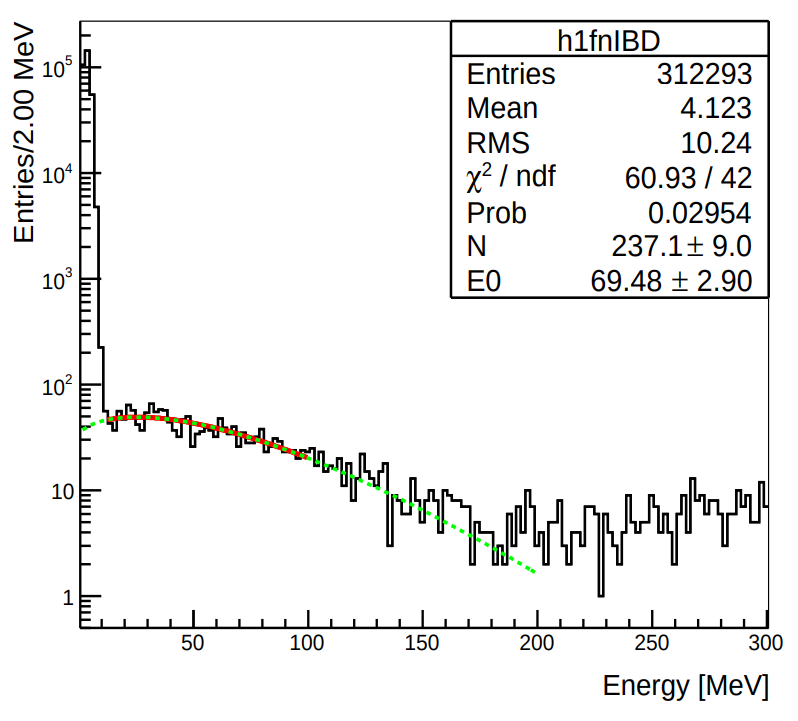
\includegraphics[width=\textwidth]{Backgrounds/FastN/ibd_fit_eh3_bz.png}%
  \end{minipage}%
  \caption{Fits of the untagged fast-neutron spectra to \autoref{eq:fastn_extrap_form} for EH1 (left), EH2 (center), and EH3 (right). From \cite{fastn}.}
  \label{fig:fastn_ibd_fit_bz}
\end{figure}

\begin{figure}[h]
  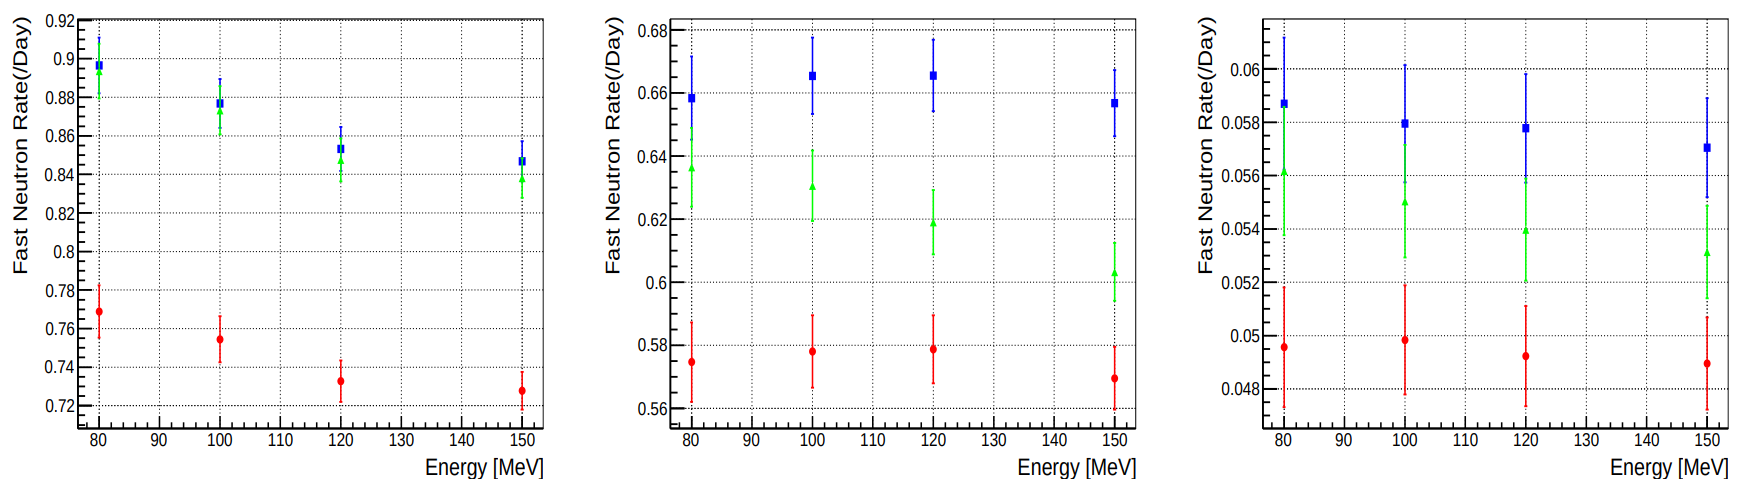
\includegraphics[width=\textwidth]{Backgrounds/FastN/rate_vs_fit_range.png}
  \caption{Daily fast-neutron rates from the extrapolation method, as a function of the upper limit of the fit range. The blue squares correspond to the IBD selection criteria used in this analysis. From \cite{fastn}.}
  \label{fig:fastn_rate_vs_fit_range}
\end{figure}

\subsection{Final result and total uncertainty}
\label{sec:fastn_comb}

In total, eight consistent estimates of \rfn\ were obtained for each hall, derived from four scaling ranges in the scaling method, and four fitting ranges in the extrapolation method \cite{fastn}. As in the official Daya Bay analysis, we arbitrarily choose the 12-100~MeV scaling method as the source of the daily fast neutron rates in this analysis.

Six uncertainties were added in quadrature to obtain the total \cite{fastn}:
\begin{itemize}
\item Statistical: The statistical uncertainty on the scaling factor $F$, described by \autoref{eq:fastn_scal_unc}.
\item Scaling range: The uncertainty from the choice of scaling range, which was determined from the difference between the highest and lowest fast-neutron rates across the four ranges used.
\item Fit range: The analogue for the choice of the fitting range.
\item Fit result: The statistical uncertainty in the fitted value of $N_\mathrm{fid}$.
\item Bin width: From the dependence of the fit results on the choice of binning, which was determined by varying the bin widths and repeating the fits.
\item Methods: From the difference in results between the scaling and extrapolation methods.
\end{itemize}
These uncertainties are summarized in \autoref{tab:bkgFastnUnc}, and the final results given in \autoref{tab:bkgFastnFinalRates}.

\begin{table}[ht]
  \begin{tabular}{lccc}
    \toprule
    Uncertainty (\%)            & EH1  & EH2  & EH3 \\
    \midrule
    Statistical & 4.6 & 5.5 & 14.7 \\
    Scaling range & 2.4 & 0.8 & 1.2 \\
    Fit range & 2.9 & 0.6 & 0.8 \\
    Fit result & 1.5 & 1.8 & 4.0 \\
    Bin width & 0.4 & 0.4 & 2.0 \\
    Methods & 7.7 & 7.7 & 7.7 \\
    \midrule
    Total & 9.8 & 9.7 & 17.2 \\
    \bottomrule
  \end{tabular}
  \caption{Uncertainty budget for the fast-neutron rates \cite{fastn}.}
  \label{tab:bkgFastnUnc}
\end{table}

\begin{table}[ht]
  \begin{tabular}{lccc}
    \toprule
    EH1 & EH2 & EH3 \\
    \midrule
    0.843 $\pm$ 0.083 & 0.638 $\pm$ 0.062 & 0.053 $\pm$ 0.009 \\
    \bottomrule
  \end{tabular}
  \caption{Final estimated fast-neutron rates (per AD per day) \cite{fastn}.}
  \label{tab:bkgFastnFinalRates}
\end{table}


\section{AmC source}
\label{sec:bkgAmC}

The first experimental suggestion of this background came from an observed excess of neutron-like (i.e. 6--12 MeV) \emph{uncorrelated} events in the top half of the detector (\autoref{fig:amc_z_dist}). Subsequent MC simulations showed that these uncorrelated events (from neutron capture in the stainless steel or the GdLS overflow tank) are associated with a correlated background. Further MC studies were then used to characterize the relationship between the rate of uncorrelated events and the rate of the correlated background.

A high-activity AmC source (HAS) was used to benchmark the MC. The HAS produced $\sim$59 neutrons/s and was enclosed in a nearly solid cylinder of stainless steel, maximizing the rate of neutron captures and inelastic scatters. It was placed on the lid of EH3-AD1 (labeled AD4) in the summer of 2012, and data was collected for ten days.

\begin{figure}[ht]
  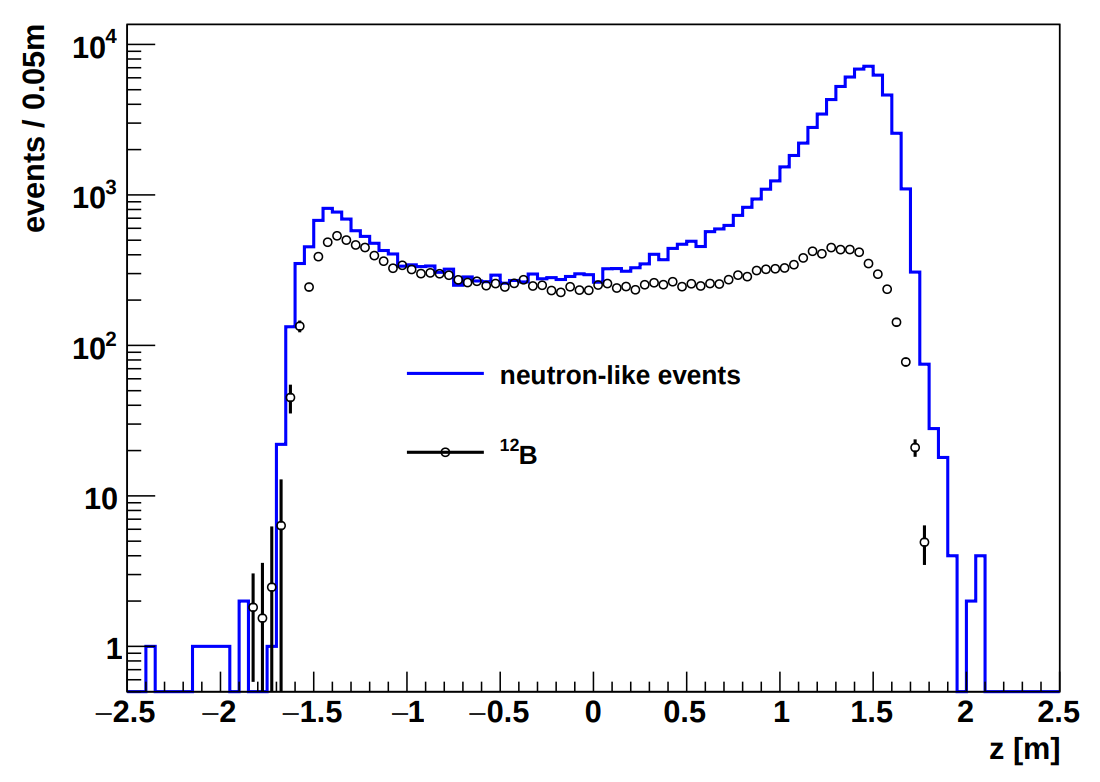
\includegraphics[scale=0.4]{Backgrounds/AmC/z_dist.png}
  \caption{Vertical distribution of uncorrelated neutron-like events, illustrating an excess in the upper half of the AD due to the AmC source in the ACUs. From \cite{Gu_2016}.}
  \label{fig:amc_z_dist}
\end{figure}

The evaluation of this AmC background is detailed in \cite{Gu_2016}. Here we briefly summarize the results, which are based on the following fundamental relationship:
\begin{equation}
  \label{eq:bkgAmcFundamental}
  R_{\mathrm{corr}} = R_{\mathrm{uncorr}} \times \xi
\end{equation}
Here, $R_{\mathrm{uncorr}}$ is the rate of uncorrelated neutron-like events produced by the AmC source (or HAS), as measured directly by taking the difference in the number of isolated neutron-like events between the top and bottom halves of each AD. Meanwhile, $\xi$ is the ratio of correlated to uncorrelated events, as determined from a combination of simulations and HAS data. All of the complexity lies in the determination of $\xi$, for which two independent estimates were made, one using HAS data, and the other using MC simulations.

\begin{figure}[ht]
  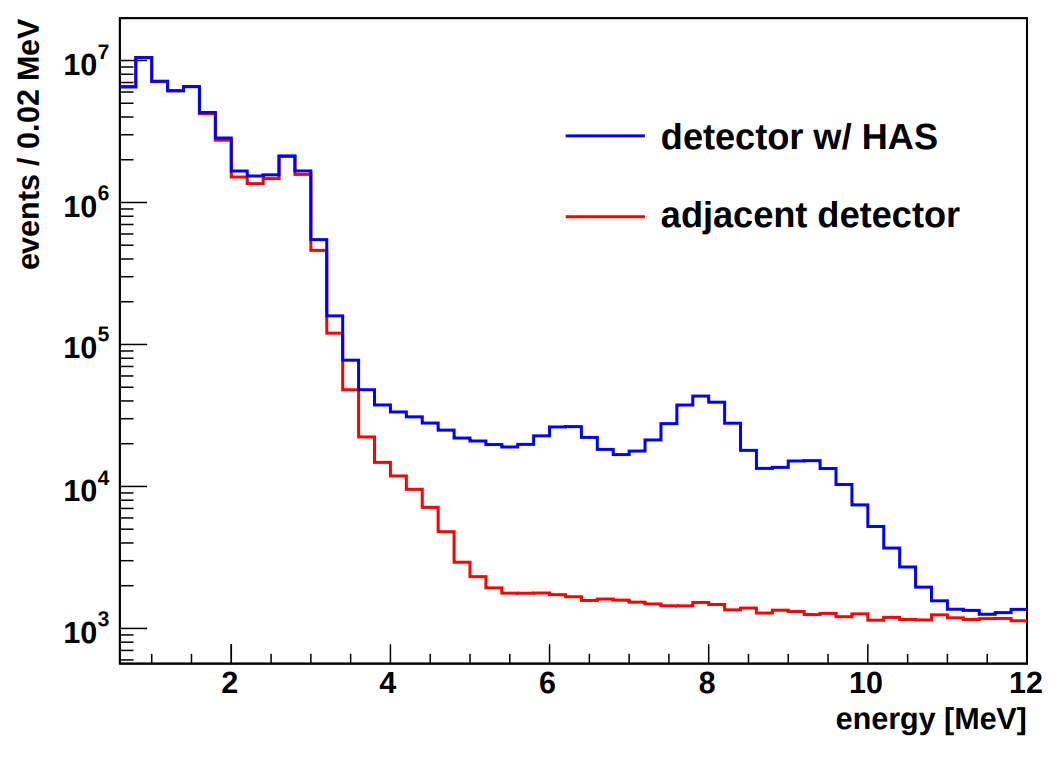
\includegraphics[scale=0.4]{Backgrounds/AmC/single_spec_2ad.png}
  \caption{Spectra of uncorrelated events (singles) in the HAS-deployed AD and an adjacent AD, showing a clear excess of neutron-like events from the HAS. From \cite{Gu_2016}.}
  \label{fig:amc_single_spec_2ad}
\end{figure}

To measure $\xi$ from HAS data, the number of uncorrelated HAS-induced neutron-like events was first determined by subtracting the neutron-like samples between AD4 (with the HAS) and the adjacent AD5, which observed $\sim$50,000 and $\sim$4,000 events, respectively (\autoref{fig:amc_single_spec_2ad}). Next, the number of \emph{correlated} HAS events was measured by taking the spectrum of IBD candidates in AD4, subtracting the accidental background, and then subtracting the (background-subtracted) IBD sample measured by AD5 (\autoref{fig:amc_prompt_spec_data}).\footnote{This procedure doesn't account for other correlated backgrounds in AD4, such as $^9$Li and fast neutrons, but their rates of $< 0.2$/d are insignificant compared to the 63 correlated events per day produced by the HAS.} The delayed spectrum from this sample, consisting of the sum of neutron-capture peaks from Fe, Ni, Cr, and Mn, demonstrated excellent agreement with the prediction of the MC, providing further validation of the MC's predictions (\autoref{fig:amc_ncap_spec_mc}). Relating the uncorrelated and correlated rates gave a value of $\xi$, \emph{for the HAS}, of $(1.5\pm0.3)\times10^{-3}$. The Geant4 MC, on the other hand, returned a $\xi$ of $(1.2\pm0.1)\times10^{-3}$ for the HAS. The 25\% difference was then assigned as the uncertainty (and bias) of the MC. With the addition in quadrature of the 20\% statistical uncertainty in the data, a total uncertainty of 30\% was assigned to $\xi$.

\begin{figure}[ht]
  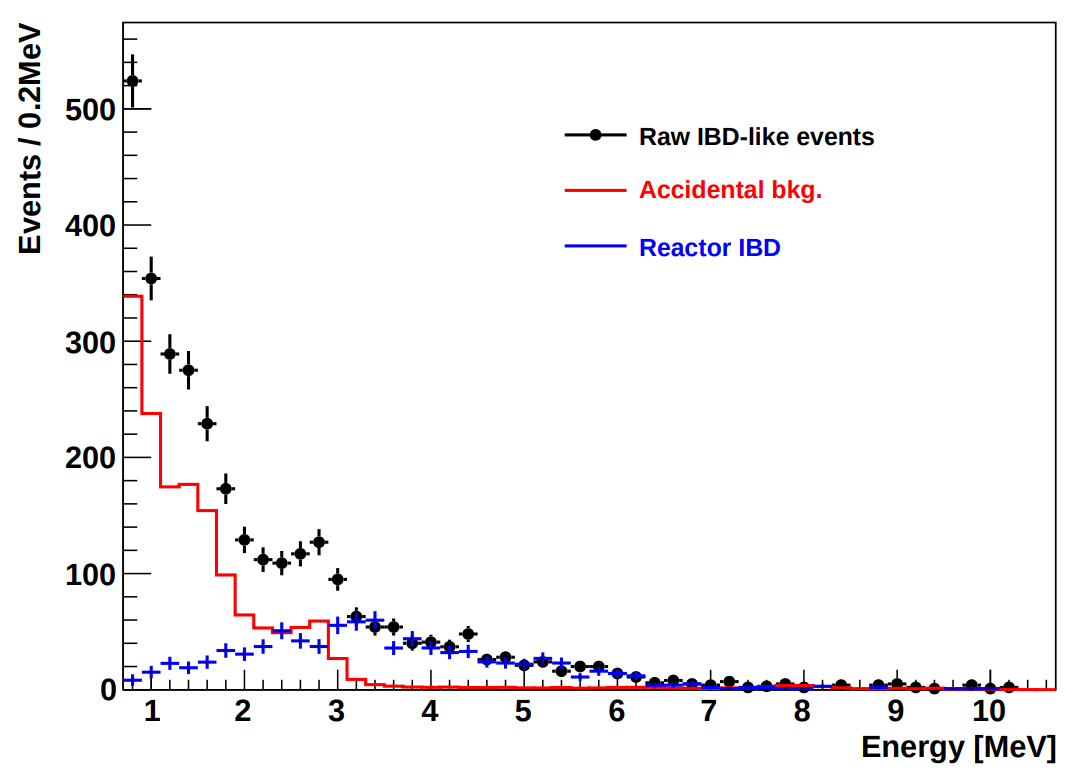
\includegraphics[scale=0.4]{Backgrounds/AmC/prompt_spec_data.png}
  \caption{Prompt spectrum of IBD-like events in the HAS-deployed detector, along with the spectrum of accidentals (determined from the singles spectrum) and the (background-subtracted) reactor IBD spectrum from an adjacent AD. From \cite{Gu_2016}.}
  \label{fig:amc_prompt_spec_data}
\end{figure}

\begin{figure}[ht]
  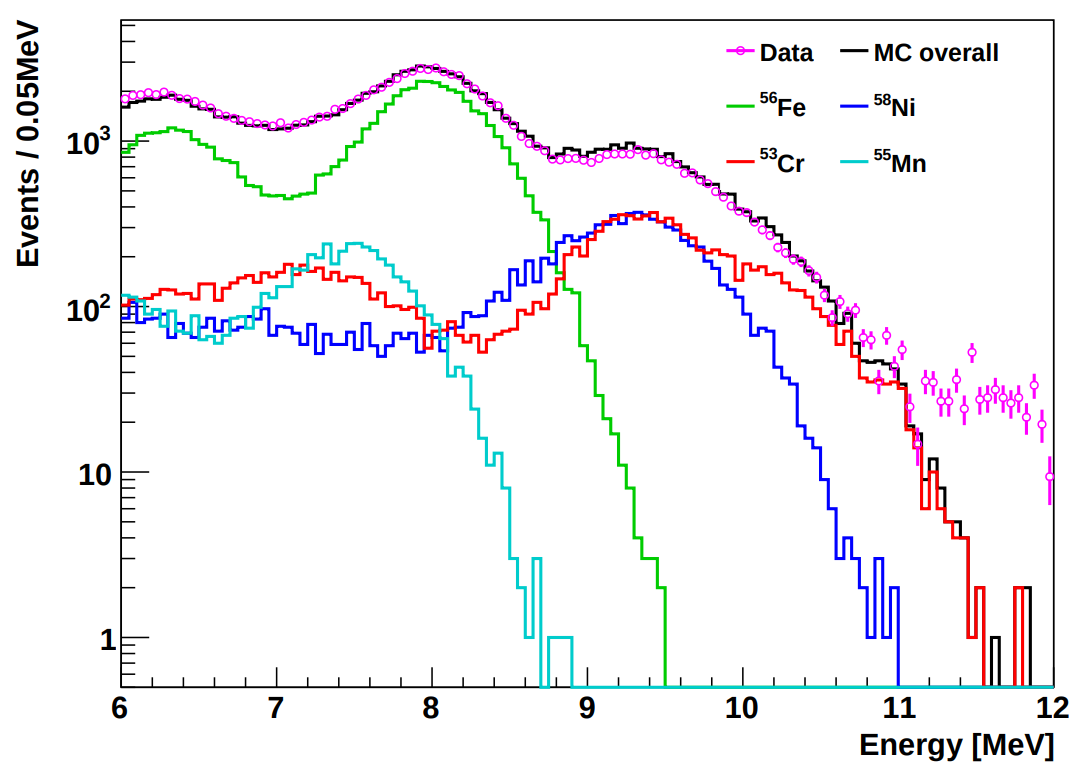
\includegraphics[scale=0.4]{Backgrounds/AmC/ncap_spec_mc.png}
  \caption{Comparison of the AmC delayed spectrum between data and the MC, showing the latter's contributions from the individual neutron capture peaks. From \cite{Gu_2016}.}
  \label{fig:amc_ncap_spec_mc}
\end{figure}

Compared to the HAS, the ordinary (low-intensity) AmC source (LAS) is expected to have a lower $\xi$, since it lies farther from the AD and has a lower density of surrounding stainless steel. For the LAS, the MC predicted a $\xi$ of $0.9\times10^{-3}$. Based on the MC/data comparison for the HAS, this value was scaled up by 25\% to $1.125\times10^{-3}$, with an uncertainty of 30\%. 

In addition to the rates, the prompt spectrum of the AmC background also required determination. Excellent agreement in the HAS prompt spectra was found between the data and MC (\autoref{fig:amc_prompt_fit_data}). Furthermore, similar agreement was found between the MC HAS and MC LAS prompt spectra (\autoref{fig:amc_prompt_fit_mc}), in spite of the differences in geometry and materials between the HAS and the LAS. As such, any one of these spectra could have been chosen as a reference. The choice was to use the measured HAS spectrum, which was fit to an exponential function,
\begin{equation}
  f(E) = p_0 \times e^{-E/p_1}.
  \label{eq:amc_fit_func}
\end{equation}
The fit gave $p_1 = \SI{0.783}{MeV}$ with a 10\% statistical uncertainty, compared to \SI{0.794}{MeV} and \SI{0.830}{MeV} for the LAS and HAS MC samples, respectively. This 5\% spread, in combination with the 10\% statisical uncertainty, gave a conservative total uncertainty of 15\% on $p_1$ (essentially a shape uncertainty). Meanwhile, $p_0$ was fixed by the normalization condition $\int f(E)\,dE = \xi$, giving (for $\xi = 1.125\times10^{-3}$) $p_0 = \SI[parse-numbers = false]{3.606\times10^{-3}}{/MeV}$. Conservatively combining the 30\% uncertainty on $\xi$ with the 15\% uncertainty on $p_1$ gave a total uncertainty of 45\% on the AmC background. Given the identical design of the ADs, identical behavior was assumed with respect to the AmC background, and no attempt was made to calculate AD-specific quantities.

\begin{figure}[ht]
  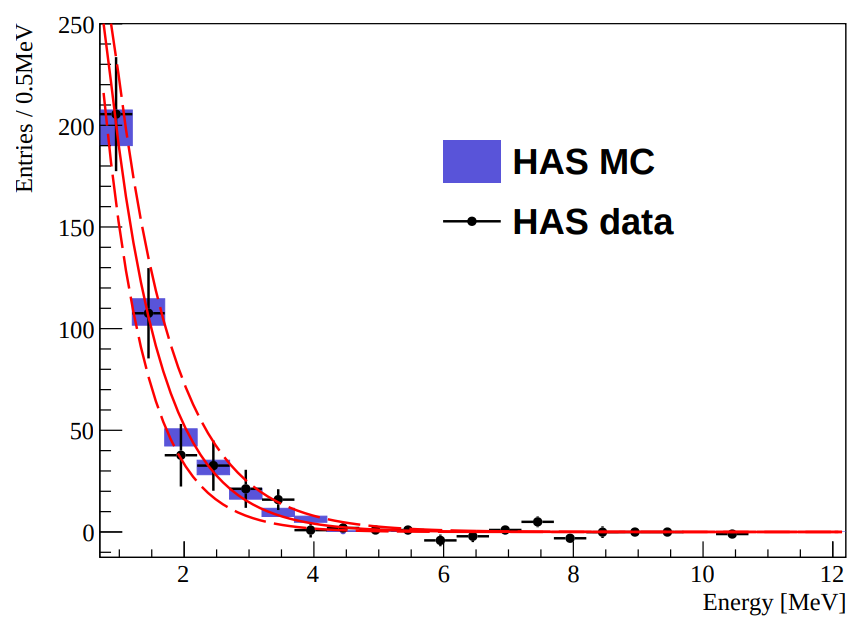
\includegraphics[scale=0.5]{Backgrounds/AmC/prompt_fit_data.png}
  \caption{Comparison of HAS prompt spectra from data and MC, showing the results of fitting the data to \autoref{eq:amc_fit_func}. From \cite{Gu_2016}.}
  \label{fig:amc_prompt_fit_data}
\end{figure}

\begin{figure}[ht]
  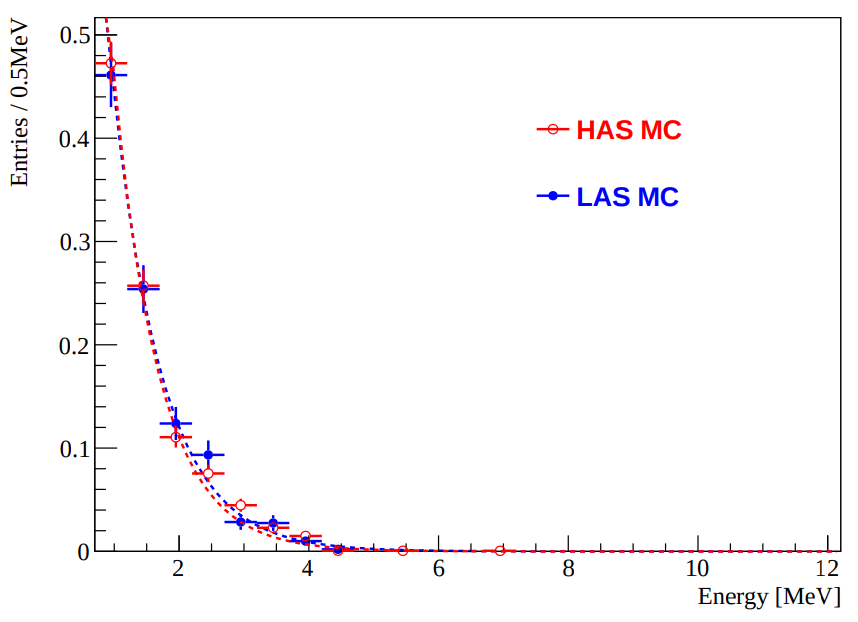
\includegraphics[scale=0.5]{Backgrounds/AmC/prompt_fit_mc.png}
  \caption{Comparison of HAS and LAS prompt spectra from the MC, showing the results of fitting the HAS spectrum to \autoref{eq:amc_fit_func}. From \cite{Gu_2016}.}
  \label{fig:amc_prompt_fit_mc}
\end{figure}

After the determination of $\xi$, the prompt spectrum (i.e. $p_1$), and the uncertainty, evaluation of each AD's AmC background then amounted to the simple task of measuring $R_{\mathrm{uncorr}}$ (after correcting for the muon veto efficiency) and multiplying it by $\xi$ according to \autoref{eq:bkgAmcFundamental}, resulting in the final values used in this analysis. It should be noted that the ACU-B and ACU-C AmC sources were removed from the EH3 ADs in 2012, during installation of EH2-AD2 and EH3-AD4.\footnote{In principle, the effective value of $\xi$ could vary between the three-sources and one-source scenarios, but this subtlety is not discussed in \cite{Gu_2016}. Presumably, any such effects fall within the 45\% uncertainty.} This significantly reduced the AmC background at the far site from 0.3\% to 0.1\% of the IBD rate. Furthermore, over the first two years of data, a 50\% decline was observed in the rate from each AmC source, in all three halls, likely due to accumulation of scintillator into the source enclosures from the weekly calibration. This led to an ultimate background rate of only 0.03\% and 0.05\%\footnote{Within the single-digit precision of these percentages, the same value is obtained regardless of whether the denominator is chosen to be the signal rate or signal+background.}, near and far, respectively (although the mean rate over the entire data sample is higher, due to the fact that earlier rates were higher---0.05\% and 0.3\%, near and far, respectively.)

For the P17B data set used in this analysis, the AmC background rates were re-estimated in \cite{lianghongBkg} using updated measurements of the uncorrelated event rates from the AmC sources. The values are listed in \autoref{tab:bkgAmcDailyRatesDetails}.

\begin{table}[ht]
  \resizebox{\textwidth}{!}{%
   \begin{tabular}{lcccccccccc}
    \toprule
    & \multicolumn{2}{c}{EH1} & & \multicolumn{2}{c}{EH2} & & \multicolumn{4}{c}{EH3} \\
    \cmidrule{2-3} \cmidrule{5-6} \cmidrule{8-11}
    Period & AD1 & AD2 & & AD1 & AD2 & & AD1 & AD2 & AD3 & AD4 \\
    \midrule
    6AD & 0.29 $\pm$ 0.13 & 0.27 $\pm$ 0.12 & & 0.30 $\pm$ 0.14 & & & 0.24 $\pm$ 0.11 & 0.23 $\pm$ 0.10 & 0.23 $\pm$ 0.10 & \\
    8AD & 0.15 $\pm$ 0.07 & 0.15 $\pm$ 0.07 & & 0.12 $\pm$ 0.06 & 0.14 $\pm$ 0.06 & & 0.04 $\pm$ 0.02 & 0.03 $\pm$ 0.01 & 0.03 $\pm$ 0.02 & 0.04 $\pm$ 0.02 \\
    7AD & & 0.11 $\pm$ 0.05 & & 0.09 $\pm$ 0.04 & 0.08 $\pm$ 0.04 & & 0.02 $\pm$ 0.01 & 0.02 $\pm$ 0.01 & 0.03 $\pm$ 0.01 & 0.02 $\pm$ 0.01 \\ 
    \bottomrule
  \end{tabular}}
  \caption{AmC background rates for the P17B data set \cite{lianghongBkg}.}
  \label{tab:bkgAmcDailyRatesDetails}
\end{table}

\section{$\CanO$}
\label{sec:bkgCanO}

Based on the chemical composition of the scintillator and the known cross sections of $\alphN$ reactions, it was determined that $\CanO$ is the only such reaction to occur in the ADs at any significant rate. Meanwhile, there are three natural decay chains that can lead to alpha-particle activity in the AD: The uranium, thorium, and actinium chains, which begin, respectively, with the long-lived isotopes $^{238}$U, $^{232}$Th, and $^{235}$U\footnote{In practice, the rate of the thorium chain is determined by the concentration of the shorter-lived $^{228}$Th ($t_{1/2}$ = 1.9~yr), and likewise, for the actinium chain by $^{227}$Ac ($t_{1/2}$ = 21.8~yr).}. Given that U, Th, and Ac all have similar chemical properties to Gd, a small amount of contamination is difficult to avoid during the Gd-doping process. In addition to these three decay chains, additional alpha particles come from the decay of $^{210}$Po, a moderately stable ($t_{1/2}$ = 138~d) daughter of $^{222}$Rn (which itself comes from the uranium chain). $^{210}$Po was deposited on detector surfaces by $^{222}$Rn during detector construction, and is essentially the only significant alpha-particle emitter outside the GdLS region.

Quantifying the $\CanO$ background consists of two parallel tasks. One task is to determine the level of alpha activity produced by the three decay chains and by $^{210}$Po. The other task is to determine, for the set of alpha particles produced by a given chain (see \autoref{fig:aln_alpha_energy_dist}), the probability and prompt spectrum of the $\CanO$ events. These two pieces of knowledge can then be combined to yield a predicted rate and spectrum for the $\CanO$ background.

\begin{figure}[ht]
  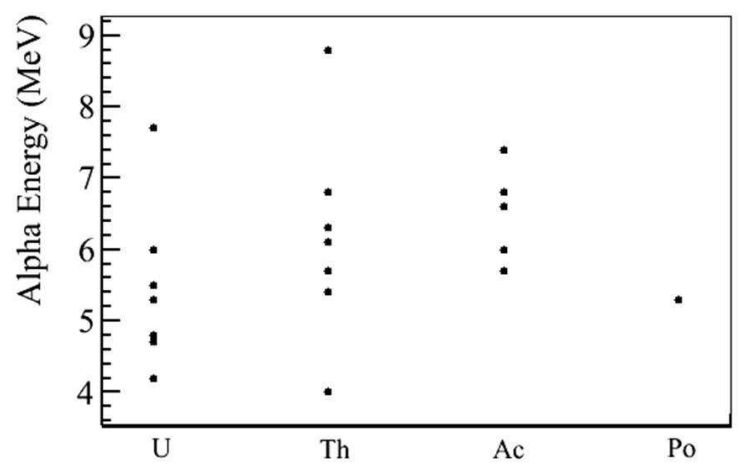
\includegraphics[scale=0.5]{Backgrounds/AlN/alpha_energy_dist.png}
  \caption{Distribution of $\alpha$ particle energies from decays of $^{238}$U, $^{232}$Th, $^{227}$Ac, and $^{210}$Po. From \cite{Zhao_2014}.}
  \label{fig:aln_alpha_energy_dist}
\end{figure}

The three chains all share a fortuitous property that enables a straightforward estimation of their rates. Namely, they each contain a rapid $\alpha$-$\alpha$ or $\beta$-$\alpha$ cascade whose time correlation and energy distribution allow for clean extraction from the data (\autoref{fig:aln_longpaper_bipo_sel}). For the uranium, thorium, and actinium chains, these cascades are, respectively, $^{214}$Bi $\to$ $^{214}$Po $\to$ $^{210}$Pb, $^{212}$Bi $\to$ $^{212}$Po $\to$ $^{208}$Pb, and $^{219}$Rn $\to$ $^{215}$Po $\to$ $^{211}$Pb, with Po half-lives of \SI{164.3}{\micro s}, \SI{0.3}{\micro s}, and \SI{1.781}{ms}, respectively.

\begin{figure}[ht]
  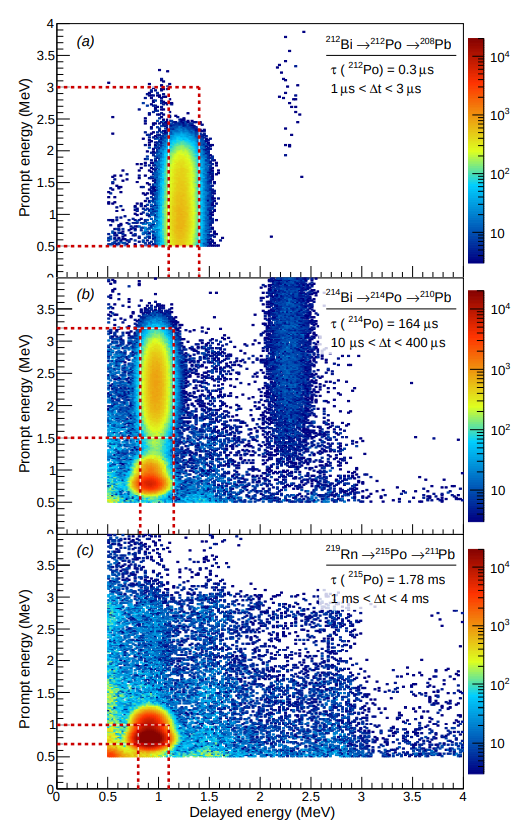
\includegraphics[scale=0.5]{Backgrounds/AlN/longpaper_bipo_sel.png}
  \caption{Illustration of the prompt and delayed energy distributions for the Bi-Po cascades used in determining the rates of the $^{238}$U, $^{228}$Th, and $^{227}$Ac decay chains. From \cite{An_2017}.}
  \label{fig:aln_longpaper_bipo_sel}
\end{figure}

To extract these events, time coincidence windows of [10, 400]~\us, [1, 3]~\us, and [1, 4]~ms were used, respectively \cite{An_2017}.\footnote{It is curious that, for the case of $^{212}$Po (i.e. $^{232}$Th), the time window used is significantly larger, relative to the half-life, compared to the other two isotopes. As shown in \autoref{fig:aln_longpaper_bipo_sel}, the $^{212}$Po sample is the ``cleanest'' (in terms of accidental backgrounds), enabling the use of a (perhaps excessively) wide window in order to maximize the statistics. Since Th is the most active chain, maximal statistics are desirable.} Accidentals (most significant for the actinium chain's Po cascade) were subtracted via the usual procedure,
% (YYY check that this was actually done, at least for actinium),
and for the uranium chain's Po cascade, contamination with nH IBDs was not an issue given that the (quenched) delayed energy of the alpha particle for these events is around 1-1.5~MeV, significantly below the 2.2-MeV gamma ray from nH capture. For the thorium chain, the prompt spectrum had to be extrapolated below 0.5~MeV in order to determine the total rate; otherwise, there were no major complications. Under the assumption that each chain is in equilibrium\footnote{Up to $^{228}$Th and $^{227}$Ac for the thorium and actinium chains, rather than all the way up to $^{232}$Th and $^{235}$U, as noted previously.}, the rate of the polonium cascade gives the rate of the entire chain.

At the point in time when Daya Bay began taking data, this procedure determined average (across ADs) rates of 0.009, 0.2, and 0.02~Bq for U, Th, and Ac, respectively \cite{lianghongBkg}. Since the U chain is initiated by $^{238}$U in the AD, its rate is essentially constant, given the $^{238}$U half-life of 4.5~Gyr. On the other hand, the Th and Ac rates do decrease over time, since the parent half-lives (i.e. those of $^{228}$Th and $^{227}$Ac) are 1.9 and 21.8~yr, respectively. To determine the average Th and Ac rates for the P17B dataset used in this analysis, the Bi-Po cascade selection was repeated, and AD-averaged rates of 0.136 and 0.0178~Bq for $^{228}$Th and $^{227}$Ac, respectively, were obtained \cite{lianghongBkg}.
% \footnote{Given the difference in half-lives between the two isotopes, one would expect a greater difference in the rate decrease than that measured by Wei. However, this discrepancy is encompassed by the uncertainty of the rate measurement procedure.}

For $^{210}$Po, a single decay instead of a chain, time correlations could not be exploited. Instead, the 5.3~MeV alpha particle produced by this isotope was, after quenching, visible as a peak around 0.5~MeV in the singles spectrum. Fitting this peak gave rates ranging from 4--10~Hz for each AD \cite{zeyuanAln}. Although the $^{210}$Po half-life is only 138 days, its parent, $^{210}$Pb (which determines the $^{210}$Po rate decrease over time), has a 22.3-year half-life. Within the precision of the measurement procedure, the decrease of the $^{210}$Po rate is effectively unobservable.

For a given decay chain (or $^{210}$Po decay), the set of emitted alpha particles is known (\autoref{fig:aln_alpha_energy_dist}). For each of these alpha particles, in turn, simulations (using Geant4 \cite{Geant4} and SRIM \cite{SRIM}) can be used to determine the rate and prompt spectrum of the $\CanO$ events. At each step in the simulation, the alpha particle loses some energy and travels some distance according to its $dE/dx$ profile in the LS. With some probability (i.e. cross section), during this step the alpha particle may be captured, producing one of the excited states of $^{17}$O. If this happens, the $^{17}$O will emit a neutron, whose energy depends on both the initial excited state of $^{17}$O and the final (excited or ground) state of $^{16}$O. The neutron produces prompt energy through proton recoils and, if it is sufficiently energetic, may scatter inelastically on $^{12}$C to produce a $\sim$5~MeV gamma ray. Additional prompt energy will come from de-excitation gamma rays if the $^{16}$O had been produced in an excited state.

The simulation calculates the (very low) probability of an $(\alpha,\mathrm{n})$ reaction occurring for a single cascade of alpha particles in a given chain (\autoref{tab:bkgAlnNeutronYield}). The simulation also produces, for the $(\alpha,\mathrm{n})$ reactions from a given chain, the 2D PDF of (a) the amount of energy deposited in the scintillator and (b) the kinetic energy of the emitted neutron (illustrated in \autoref{fig:aln_energy_pdf}). Finally, the prompt-energy spectrum (\autoref{fig:aln_longpaper_prompt_spec}) is obtained by sampling this PDF and performing MC simulations of the detector's response to the alpha particle, the neutron's recoil protons, and any gamma rays from $^{12}$C inelastic scattering and $^{16}$O$^*$ de-excitation.

\begin{table}[ht]
  \begin{tabular}{lcccc}
    \toprule
    Chain & $N_{\mathrm{ground}}$ & $N_{\mathrm{excited}}$ & $N_{\mathrm{total}}$ & Uncertainty  \\
    \midrule
    $^{210}$Po & $5.26\times10^{-8}$ & $4.90\times10^{-9}$ & $5.75\times10^{-8}$ & 7.2\%  \\
    $^{238}$U  & $4.34\times10^{-7}$ & $2.96\times10^{-7}$ & $7.30\times10^{-7}$ & 16.9\% \\
    $^{228}$Th & $4.49\times10^{-7}$ & $4.92\times10^{-7}$ & $9.41\times10^{-7}$ & 27.7\% \\
    $^{227}$Ac & $4.72\times10^{-7}$ & $6.18\times10^{-7}$ & $1.09\times10^{-6}$ & 25.9\% \\
    \bottomrule
  \end{tabular}
  \caption{Neutron yield (i.e., number of $(\alpha,\mathrm{n})$ events) per decay chain. $N_{\mathrm{ground}}$ and $N_{\mathrm{excited}}$ refer to the number of events that leave $^{16}$O in the ground and excited states, respectively. $N_{\mathrm{total}}$ is their sum, whose uncertainty is given in the final column. From \cite{Zhao_2014}.}
  \label{tab:bkgAlnNeutronYield}
\end{table}

\begin{figure}[ht]
  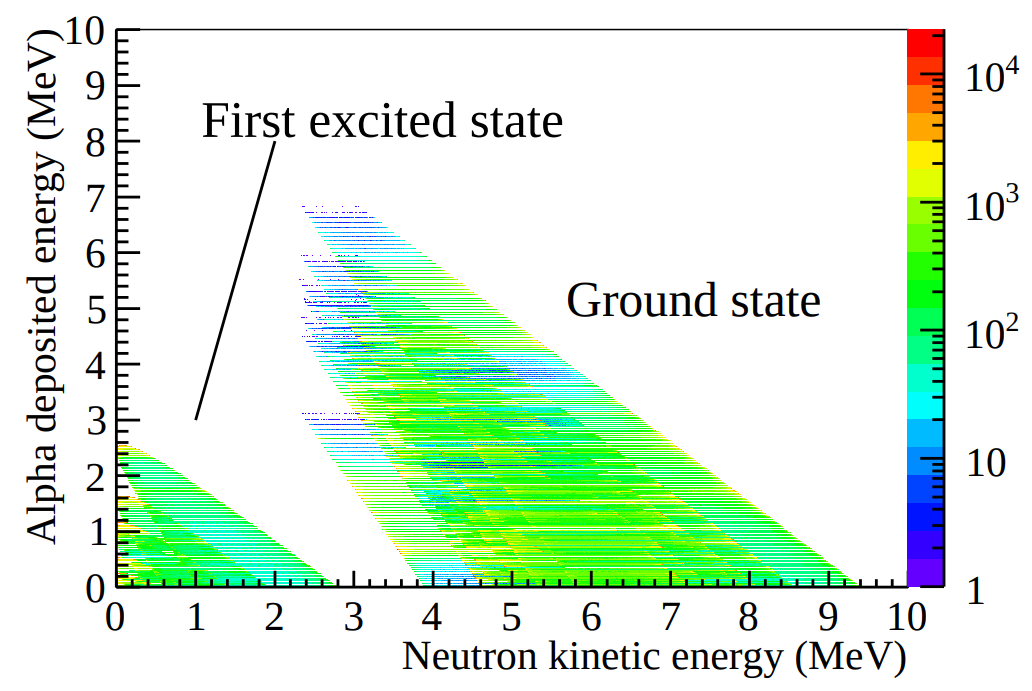
\includegraphics[scale=0.45]{Backgrounds/AlN/energy_pdf.png}
  \caption{Probability distribution function of alpha-particle energy deposition and neutron kinetic energy for $(\alpha,\mathrm{n})$ reactions from the $^{228}$Th chain. From \cite{Zhao_2014}.}
  \label{fig:aln_energy_pdf}
\end{figure}

\begin{figure}[ht]
  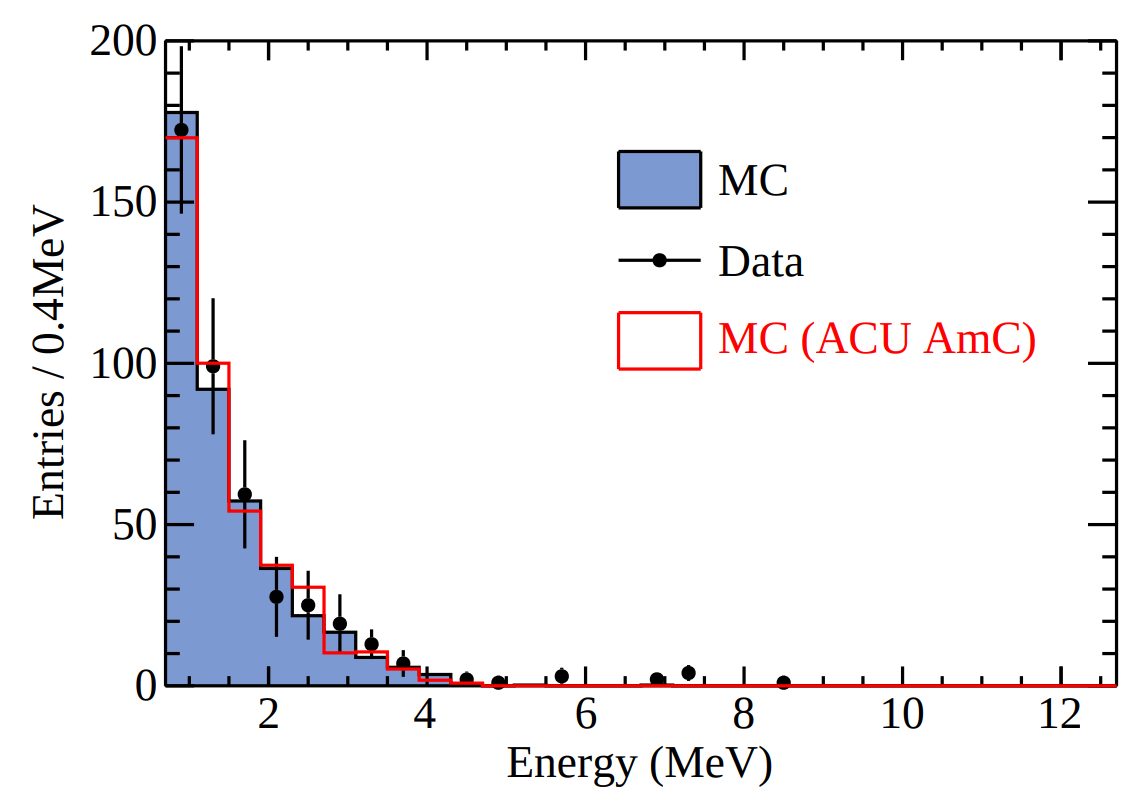
\includegraphics[scale=0.5]{Backgrounds/AlN/longpaper_prompt_spec}
  \caption{Simulated prompt-energy spectra for $(\alpha,\mathrm{n})$ reactions produced by the four decay chains. From \cite{An_2017}.}
  \label{fig:aln_longpaper_prompt_spec}
\end{figure}

Uncertainties in the $\CanO$ prediction arise from a number of sources. The uncertainty coming from the $\alphN$ cross section was estimated by repeating the MC procedure using two different cross-section tables, JENDL \cite{jendl} and EXFOR \cite{exfor} (\autoref{fig:aln_xsec}). This suggested an uncertainty ranging from 6.6\% (for $^{210}$Po) up to 27.5\% (for $^{232}$Ac) \cite{Zhao_2014}; a nominal uncertainty of 20\% was thus assigned. Meanwhile, there was negligible effect on the predicted neutron reconstructed energy spectrum from switching between the cross-section tables and from changing the assumed neutron angular distribution (\autoref{fig:aln_n_vis_spectra}). Additional uncertainty could come from the fundamentals of the MC simulation, i.e., the $dE/dx$ table and the numerical integration of discrete steps. This was evaluated by comparing the results of Geant4 \cite{Geant4} and SRIM \cite{SRIM} (\autoref{fig:aln_n_kin_spectra}), which differed, overall, at a negligible level of less than a percent. Finally, the assumption of decay-chain equilibrium, and the efficiency of the cascade selection, both could introduce additional uncertainty, leading to the conservative assignment of an overall 30\% uncertainty\footnote{Presumably validated by varying the Bi-Po cascade selection criteria, although this is not explicitly stated in the references.} in the measurement of the rates of the decay chains. This 30\% uncertainty is combined with the 20\% uncertainty assigned to the neutron yield calculation; conservatively adding the two uncertainties then gives a total uncertainty of 50\% on the $\CanO$ rate estimation.

\begin{figure}[ht]
  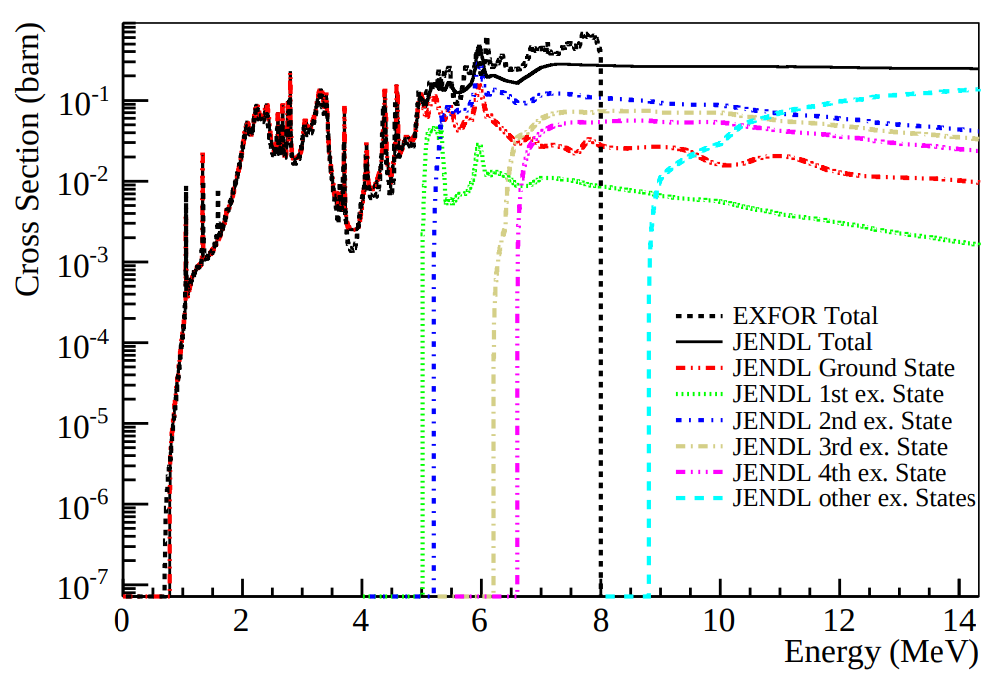
\includegraphics[scale=0.5]{Backgrounds/AlN/xsec.png}
  \caption{Cross section of the $\CanO$ reaction as reported by the JENDL and EXFOR tables. From \cite{Zhao_2014}.}
  \label{fig:aln_xsec}
\end{figure}

\begin{figure}[ht]
  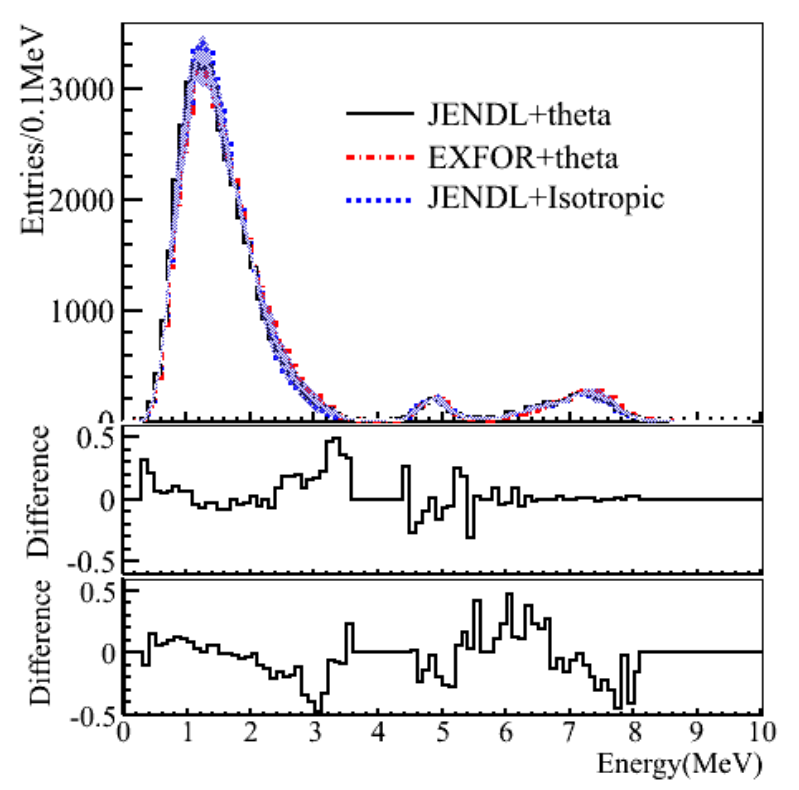
\includegraphics[scale=0.5]{Backgrounds/AlN/n_vis_spectra.png}
  \caption{Predicted reconstructed energy of neutrons for different cross-section tables (JENDL and EXFOR) and different neutron angular distributions (``theta'', $d\sigma/d\Omega \sim 1/\sin\theta$, and ``isotropic'', $d\sigma/d\Omega \sim 1$). The differences are negligible. From \cite{Zhao_2014}. (The particular decay chain is not specified.)}
  \label{fig:aln_n_vis_spectra}
\end{figure}

\begin{figure}[ht]
  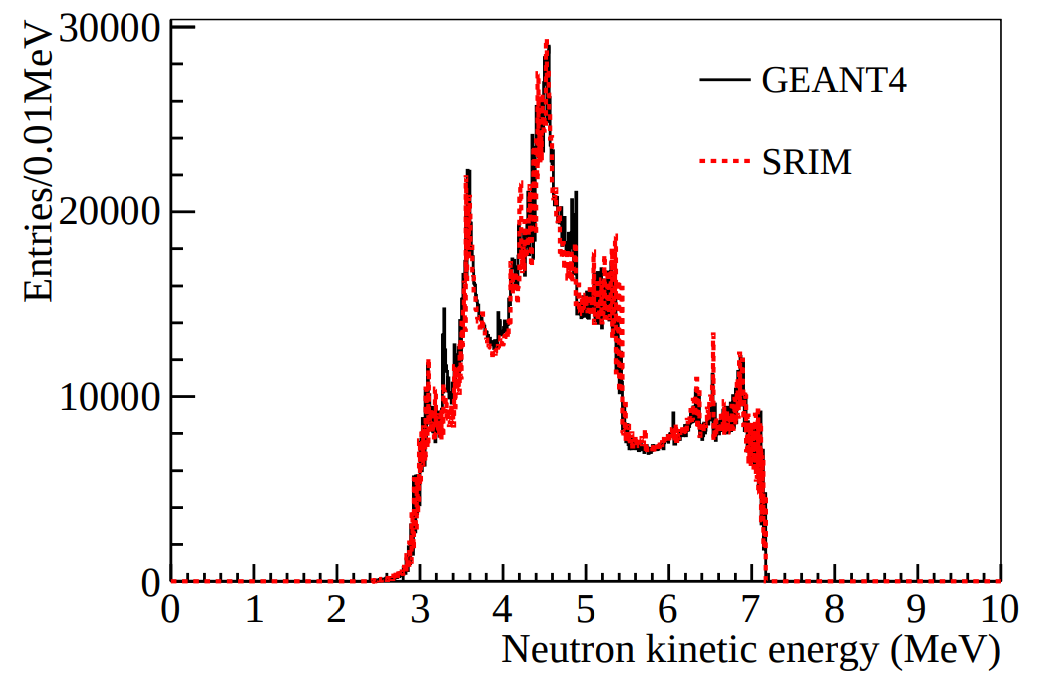
\includegraphics[scale=0.45]{Backgrounds/AlN/n_kin_spectra.png}
  \caption{Neutron kinetic energy as predicted by Geant4 and SRIM. From \cite{Zhao_2014}. (The particular decay chain is not specified.)}
  \label{fig:aln_n_kin_spectra}
\end{figure}

For the P17B data set used in this analysis, the $\CanO$ background rates were re-estimated using updated measurements of the rates of alpha activity \cite{lianghongBkg}. The values are listed in \autoref{tab:bkgAlnDailyRates}.

\begin{table}[ht]
  \resizebox{\textwidth}{!}{%
    \begin{tabular}{lcccccccccc}
      \toprule
      & \multicolumn{2}{c}{EH1} & & \multicolumn{2}{c}{EH2} & & \multicolumn{4}{c}{EH3} \\
      \cmidrule{2-3} \cmidrule{5-6} \cmidrule{8-11}
      Period & AD1 & AD2 & & AD1 & AD2 & & AD1 & AD2 & AD3 & AD4 \\
      \midrule
      6AD & 0.09 $\pm$ 0.04 & 0.07 $\pm$ 0.04 & & 0.05 $\pm$ 0.02 & & & 0.05 $\pm$ 0.02 & 0.04 $\pm$ 0.02 & 0.04 $\pm$ 0.02 & \\
      8AD & 0.08 $\pm$ 0.04 & 0.06 $\pm$ 0.03 & & 0.04 $\pm$ 0.02 & 0.06 $\pm$ 0.03 & & 0.04 $\pm$ 0.02 & 0.04 $\pm$ 0.02 & 0.03 $\pm$ 0.02 &  0.04 $\pm$ 0.02 \\
      7AD & & 0.05 $\pm$ 0.03 & & 0.03 $\pm$ 0.02 & 0.06 $\pm$ 0.03 & & 0.03 $\pm$ 0.02 & 0.03 $\pm$ 0.02 & 0.03 $\pm$ 0.01 & 0.03 $\pm$ 0.02 \\
      \bottomrule
    \end{tabular}}
  \caption{$\CanO$ background rates for the P17B data set \cite{lianghongBkg}.}
  \label{tab:bkgAlnDailyRates}
\end{table}

\subsection{Efficiencies}
\label{sec:bkgFlasherEffs}

The exact efficiency of these cuts (i.e., the rejection factor for flashers), is unimportant, as long as it is high enough.\footnote{According to \cite{SideBySide}, the efficiency is greater than $99.99\%$.} Any residual flashers will automatically be counted in the singles rate, and thus so will their contribution to the accidental background rate.\footnote{There is a small second-order correction due to the fact that an accidental cannot be formed by two flashers in the same PMT, given that it takes on the order of a second for a PMT to ``recharge'' after flashing. However, this correction is negligible given the extremely low rate of residual flashers.} As shown in \autoref{fig:fID_dist}, the rejection factor (and hence the purity of the IBD sample, with respect to flashers) is very nearly 100\% in all ADs, with the minor exception of AD5, where the small contribution of unrejected flashers will, in any case, be removed during the subtraction of the accidental background spectrum.

Compared to the efficiency, it \emph{is} important to study the signal inefficiency, i.e. the probability of improperly rejecting an IBD prompt or delayed trigger. If this inefficiency differs significantly among the ADs, it could bias the oscillation result.
% The inefficiency was estimated \cite{xinFlasherEff1,xinFlasherEff2} by taking a sample of IBD-like events (without the flasher cut), and making a 2D histogram of $(f_{\mathrm{prompt}},f_{\mathrm{delayed}})$, where $f$ is $\fID$ or $\fPSD$. The IBD-like sample consists of a small number of accidentals that contain a flasher (or two), and a much larger number of flasher-free pairs (including true IBDs, accidentals, and correlated backgrounds). The use of IBD-like events has the effect of diluting the presence of flashers in the sample, since a coincident pair is much more likely to come from an IBD than an accidental (which furthermore is more likely to have two physical singles rather than a flasher). The inefficiency was then determined by the degree to which the flasher-free ``blob'' extended into the regions rejected by the discriminator. These studies found that $\fID$ and $\fPSD$ each introduce a maximum inefficiency of 0.02\%, with uncertainties of 0.01\% correlated and 0.01\% uncorrelated.
%% From these studies, the efficiency of the flasher cut (when applied to true IBDs) was determined to be 99.98\% $\pm$ $0.01\%$ (correlated) $\pm$ $0.01\%$ (uncorrelated) \cite{An_2017}.
The inefficiency was estimated \cite{patrickFlashers} using a $\sim$600-day sample of IBD-like events (without any flasher cuts). For each of the three flasher discriminators (2", $\fID$, and $\fPSD$), a 2D histogram was constructed of its values for the prompt and delayed events. These histograms indicated that essentially all rejected IBDs had a flasher-like prompt (but not delayed) trigger. Accordingly, 1D histograms were then constructed of the discriminators of the prompt triggers for all pairs that lacked a flasher-like delayed trigger. Near the region of overlap between the IBD and flasher distributions, the true IBD distribution was fit (to both exponential and Gaussian functions) and extrapolated in order to estimate the fraction within the rejection region (\autoref{fig:flasher_fID_extrap}). Systematic uncertainties were determined by varying the fit range and function. These results were then cross-checked by exploiting the different prompt-delayed time correlations of the two event classes, giving an independent breakdown of the total distribution into its IBD and flasher components (\autoref{fig:flasher_fID_time}). The total inefficiency was found to be $0.039\% \pm 0.006\%$, as summarized in \autoref{tab:flasher_ineff}. AD-to-AD variations lay within this uncertainty band.

\begin{figure}[ht]
  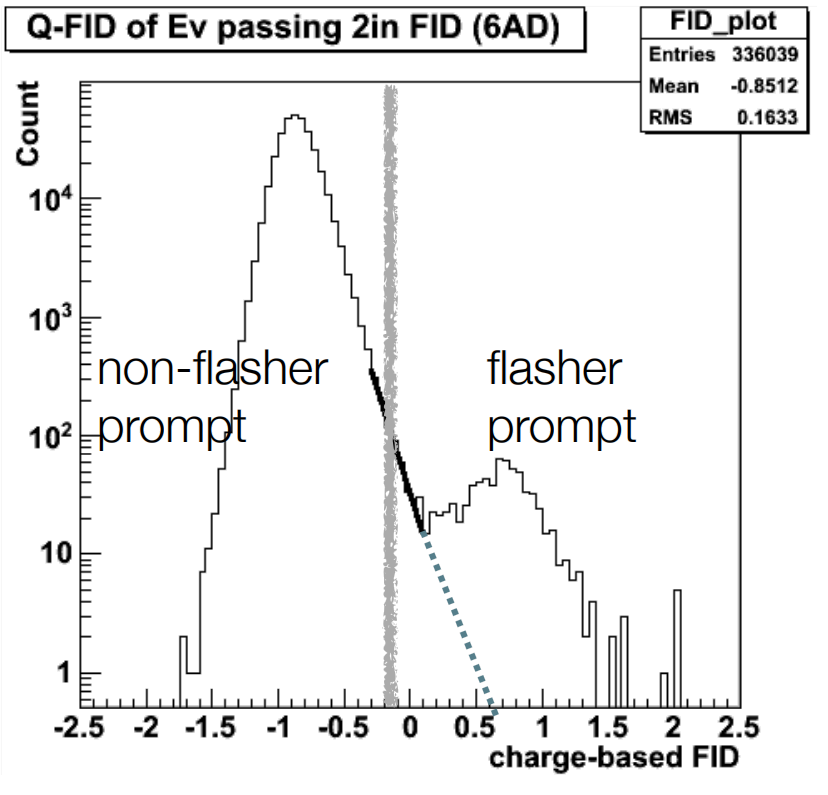
\includegraphics[width=0.5\textwidth]{Backgrounds/Flasher/ineff_fID_extrap.png}
  \caption{The prompt $\fID$ distribution of IBD-like events for which the delayed trigger is \emph{not} flasher-like (as determined by $\fID$). The true IBD component is fit and extrapolated in order to determine the inefficiency of the cut. From \cite{patrickFlashers}.}
  \label{fig:flasher_fID_extrap}
\end{figure}

\begin{figure}[ht]
  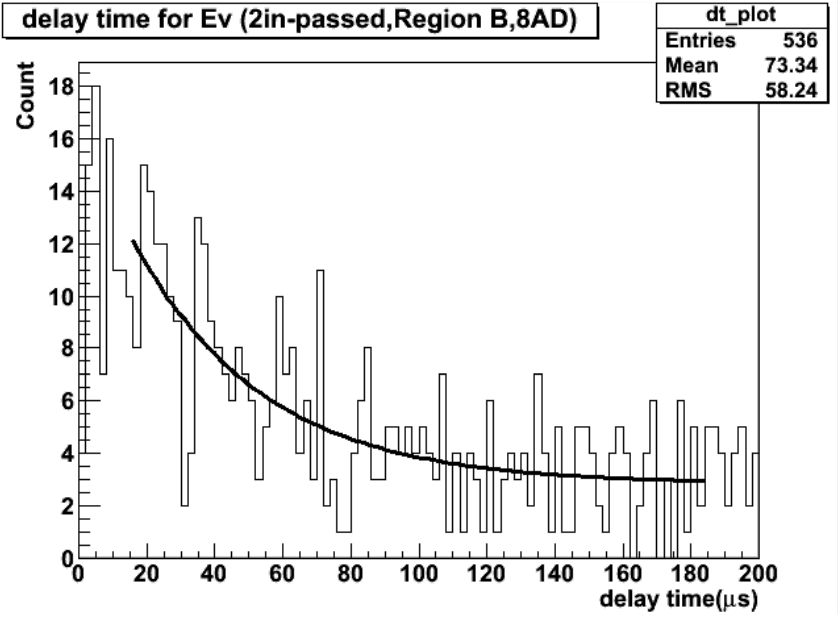
\includegraphics[width=0.5\textwidth]{Backgrounds/Flasher/ineff_fID_time.png}
  \caption{The prompt-delayed time difference of IBD-like events for which the delayed trigger is \emph{not} flasher-like (as determined by $\fID$). The true IBD component follows an exponential distribution, while the flasher component is flat. A fit is performed in order to quantify the two components. From \cite{patrickFlashers}.}
  \label{fig:flasher_fID_time}
\end{figure}

\begin{table}[ht]
  \begin{tabular}{lc}
    \toprule
    Cut & Inefficiency (\%) \\
    \midrule
    2" PMT  & $0.000 \pm 0.000$ \\
    $\fID$  & $0.023 \pm 0.004$ \\
    $\fPSD$ & $0.016 \pm 0.002$ \\
    \midrule
    Total & $0.039 \pm 0.006$ \\
    \bottomrule
  \end{tabular}
  \caption{Inefficiencies of the flasher cuts \cite{patrickFlashers}. For true IBDs, the distributions of the three discriminator were assumed to be uncorrelated, so that the total inefficiency was determined as the sum of the three. The systematic uncertainties were conservatively assumed to be fully correlated, and were thus added linearly rather than in quadrature.}
  \label{tab:flasher_ineff}
\end{table}


% We use both cuts in our analysis. Given that the two cuts are based on different information (charge and time), we assume that our estimated inefficiency is 0.04\%, with an uncertainty of 0.02\% correlated and 0.02\% uncorrelated.

\end{document}